% Created by Carlo Occhiena, 2023
% Engine: XELATEX
% Version: TeX 2019

\documentclass{article}

% PACKAGES
\usepackage[utf8]{inputenc}
\usepackage[english]{babel}
\usepackage{amsmath} % provides many mathematical environments & tools
\usepackage{amssymb} % to display \varnothing symbol
\usepackage{array} % to manage table alignment
\usepackage{changepage} % dynamically change a page layout
\usepackage{geometry} % to manage dynamic page layout
\usepackage{graphicx} % to handle images
\usepackage{makecell} % to manage multiline cells
\usepackage[document]{ragged2e} %% to manage text alignment
\usepackage{parskip} % to manage paragraph spacing
\usepackage{fancyhdr} % to manage page header and footer

% this has to be the last package ever  
\usepackage{hyperref} % clickable URLs

\graphicspath{ {./images/} } % tells the program what folder to find the images in

% USER CUSTOMIZATION
\renewcommand{\arraystretch}{1.5} % add height to tables

% FUNCTIONS 

% DOCUMENT CUSTOMIZATION
\title{The Statistics Handbook \\ 
    \normalsize Version 0.1}
\author{ Carlo Occhiena }
\date{ Jan 2023 }


\begin{document}

% CUSTOM HEADER
\fancyhead{}
\setlength{\headheight}{13.6pt}
\pagestyle{fancy}
\rhead[]{\rightmark} % section name

\maketitle
% \centerline \LaTeX{}
\tableofcontents
\clearpage

\section{Scope of this handbook}
We are used to talking generally about mathematical skills, thinking perhaps of derivatives, integrals, theorems, and graphs of functions. 

Often we do that in an abstract way, as if they were certainly logical elements, but with just specific applications. Instead, we forget that not only are mathematical elements present in every single action, but that quantitative sciences are components of everyday life.

Specifically, I believe that statistics is among all the mathematical sciences the most fascinating because of the vastness and incredible opportunities for its application. 

Every decision we make can be traced back to statistical phenomena, either innate (such as fear of the dark, because in the dark increases the likelihood of dangerous animals) or conscious (today I think it's likely to rain, so I'll take my umbrella). 

On the other hand, approaching even basic statistical calculations (e.g., the infamous probability of winning the lottery) requires nontrivial skills in order to apply concepts and formulas that are not always complex but certainly have dissimilar results if used thoughtlessly. I claim for certain that worse than the lack of mathematical thinking is the misuse of mathematical thinking. This paper of mine is also in fact intended to combat my limitations through study and applications. 

In this handbook, I wanted to create a path from the basics, including terminology (often one of the main obstacles for the laymen approaching the subject), to formulations of hypotheses, validations, and verification of formulas.

The path was constructed by consulting a large number of sources, cited in the appendix, and during long months of study and in-depth proof of the results and evidence, precisely because first and foremost I wanted to verify my own expertise, even before, of course, I could write about it. 

Before releasing this publication, which is distributed under a Creative Common and Free Culture license, I asked for a check from eminent acquaintances with important academic and working backgrounds. I would like to endlessly thank all of them (their names can be found in the appropriate section). Nevertheless, I am staying receptive to additions, insights and corrections, taking full responsibility for any shortcomings and errors, certainly reported in good faith.

Happy reading! 

Carlo, 4th of January 2023.

\subsection{Versioning \& Contributions}
\begin{itemize}
    \item Version 0.1 is the first release ever published and distributed online. It's the version written and verified personally by me but does not include any third-party contributions or revisions. 
    \item I plan to submit the handbook to several SME (Subject Matter Experts). 
    \item Each contribution will be indicated in the Acknowledgments section. 
    \item The feedback from each SME will help raise the version by 1/10, so that with 9 revisions it will progress to version 1.0 of the document.
    \item Contributions are free and welcome, you can contact me via \href{https://www.linkedin.com/in/carloocchiena/}{Linkedin}. 
\end{itemize}


\subsection{\LaTeX{} \& Open Source Repository}
In addition to being distributed under a Free Culture CC BY 4.0 license, all materials related to this handbook are available in the GitHub repository at the link: \href{https://github.com/carloocchiena/the_statistics_handbook}.

This also includes the \LaTeX{} source of this handbook and an Excel with several exercises and applied formulas. This could therefore also be helpful to students and those who want to use this handbook for practical purposes. 

\clearpage

\section{Core Concepts}
\subsection{Let's start from a question}
“What is data?”

Data are collected observations and information about a given phenomenon.

“What is statistics?”

Statistics Is the discipline that concerns the collection, organization, analysis, interpretation, and presentation of data.

“What is a statistical variable?”

It’s the specific characteristic being analyzed among the statistical units on which the statistical analysis is focused on, such as “age” from all the data that may be related to the object “person”. Classification of variables and their measure of scale is paramount to set up the analytical process of statistical analysis. 

\subsection{Property and type of data}

We should not think that the data is solely a numerical value. There is a multitude of data types, each with specific characteristics. 

\subsubsection{Continuous vs Discrete}
Discrete means it can only take certain values. There are no “in-between” values. 

Discrete data is the number of people: there could be 1 person or 2 people, but not 1,5 people or 0,99 people. 
Discrete data are the possible value of rolling a die: 1,2,3,4,5,6 and not 6.5 or 1.5

Continuous means there is an infinite amount of value in between each data point.

Continuous data is the height or weight of a person.
Continuous data are temperature records. 
 
\subsubsection{Nominal vs Ordinal}
Nominal data is classified without a natural order or rank. Nominal data can’t be clearly sorted. 
Nominal data can’t be “ordered” (from which the term “ordinal”).

Nominal data are animal species: lizard, dog, cat, or the list of ingredients on a recipe.

Ordinal data is data that has a natural order or rank. 
Ordinal data can be sorted and ordered. 
Ordinal data doesn’t have to be numeric. For example, hot, mild, cold - or even top, low, bottom, can be data attributes that can be ordered and then being considered ordinal. 
Ordinal data are the seat numbers on a train. 

\subsubsection{Structured vs Unstructured}
Structured data is highly specific and stored in a predefined format. It has its own structure.
Examples are JSON or Excel files, SQL databases. 

Unstructured data is data that does not have a specific or well defined format. 
Unstructured data are audio data, text data, video data. 

Do not confuse “file format” with “formatted data”. 
Just because text is in a PDF format doesn't make it structured data. 

\subsubsection{Statistical Variables and their properties}

\paragraph{Qualitative Statistical Variables}\mbox{} \\
\mbox{} \\

Qualitative statistical variables are variables whose values are not numbers but modes, or categories. 

Examples are: “male” or “female”, “education”, “marital status”, “ethnicity” and such.

Those categories have to be exhaustive and mutually exclusive - a datapoint can’t be both “male” and “female” or both “asian” and “european”. This is a specific problem that may occur in the data preparation and data gathering phase. 

Qualitative statistical variables can be classified further in:

\textbf{Dichotomic:} variables that have only two kinds of mutually exclusive categories,  such as “male” or “female” or “alive” or “dead”.

\textbf{Nominal:} variables that have no logical order, are not comparable and not exclusive to each other. Examples of nominal variables are “transportation used for work” or “sport played”.

\textbf{Ordinal:} variables that have a logical predefined order, but yet can’t be classified as quantitative. 
Example is “education”; High School is surely lower than University, but of how much? 
And how far is a MsC from a PhD? They are clearly different, but this difference can’t be clearly measured. 

    \begin{itemize}
        \item \textbf{Linear ordinal:} they have a clear start and end, such as size “S M L XL”.
        \item \textbf{Cyclical ordinal:} they have no clear start and end and their order is based on convention (such as week days: weeks starts both on Monday, or on Sunday. Seasons).
    \end{itemize}

\paragraph{Quantitative statistical variables}\mbox{} \\
\mbox{} \\

Quantitative statistical variables are expressed by a numerical quantity.
Quantitative data is naturally ordinable and comparable. 

Quantitative data can be further classified in: 

    \begin{itemize}
        \item \textbf{Interval data:} datapoint are expression of a specific point of the dataset (such as result of a test, QI, temperature).
        \item \textbf{Ratio scale data:} data that is expressed by a rate, such as age and weight.
    \end{itemize}

\paragraph{Parametric vs Nonparametric}\mbox{} \\
\mbox{} \\

\textbf{Parametric}
\begin{itemize}
    \item Parametric assume the presence of distributions of approximately normal type.
    \item They involve continuous or interval-type variables and a fairly large sample size.
    \item They assume homogeneity of variances (homoscedasticity).
    \item They assume estimation of parametric data such as mean, variance and standard deviation.
\end{itemize}

Parametric tests have higher statistical power because they provide a higher probability of correct rejection of an incorrect statistical hypothesis. 

\textbf{Nonparametric}\mbox{} \\
Nonparametric doesn’t imply any kind of distribution and doesn’t imply any kind of parametric estimation such as mean, variance and standard deviation (because, for example, such measures are not estimable).

Nonparametric tests should be preferred whenever the dataset is not distributed in a normal (gaussian distribution) way, or, in any case, this specificity is not being demonstrated. A typical example is whenever the dataset is too small to prove a parametric distribution.

\paragraph{Homoscedasticity vs Heteroscedasticity}\mbox{} \\ 
\mbox{} \\

\textbf{Homoscedasticity} means that all random variables in the dataset have the same finite variance.

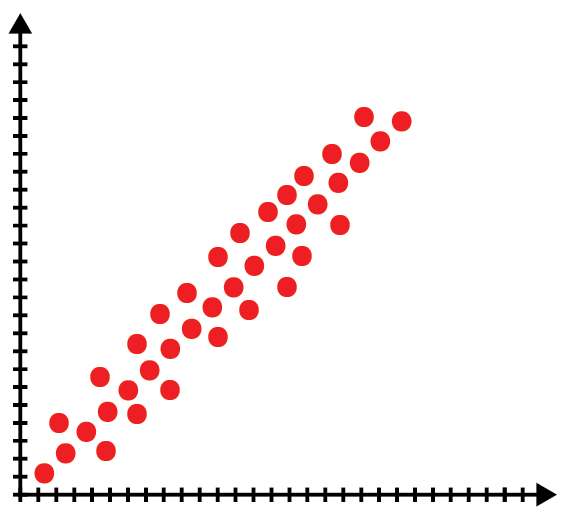
\includegraphics[width=3cm, height=3cm]{homoscedasticity}

\textbf{Heteroscedasticity}  means that not all random variables in the database have the same finite variance.

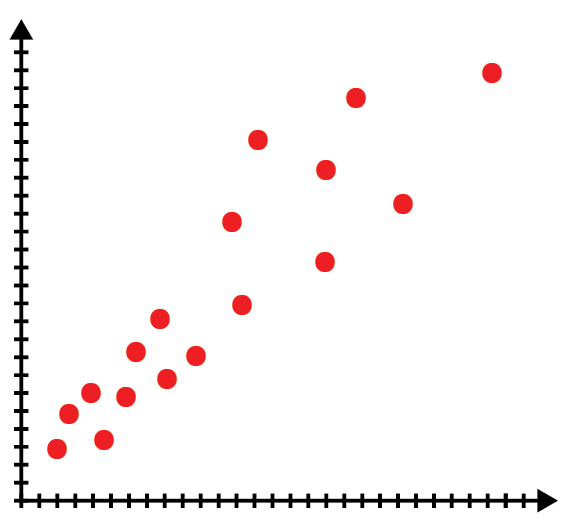
\includegraphics[width=3cm, height=3cm]{heteroscedasticity}

\paragraph{Linear, Nonlinear, and Monotonic Relationships}\mbox{} \\ 
\mbox{} \\

\textbf{Linear}: \\ 
When variables increase or decrease concurrently and at a constant rate, a positive linear relationship exists.
When one variable increases while the other variable decreases, a negative linear relationship exists.

\textbf{Nonlinear}: \\
If a relationship between two variables is not linear, the rate of increase or decrease can change as one variable changes, causing a "curved pattern" in the data.

\textbf{Monotonic}: \\
In a monotonic relationship, the variables tend to move in the same relative direction, but not necessarily at a constant rate.

\subsection{Population vs Sample}

\textbf{Population} consists of the representation of every member of a given group or of the entire available data set.
Examples are all the students of a class or all the animals of a specific national park.

\textbf{Sample} refers to a subset of the entire data set. 
For example, the first 10 students of a class or the top 3 predators from a specific national park.

Population and Sample are data definitions that are heavily dependent from the context.

When analyzing data related to a population, it is necessary to include a statistically relevant sample. A representative sample. 
Sample sizes are a well studied science. 
For example 300 is a representative sample out of a population of 1000 students.

Use “population” when:
\begin{itemize}
    \item It’s known the dataset is related to the entire population.
    \item A generalization to a wider, larger population is not interesting.
\end{itemize}

Use “sample” when:
\begin{itemize}
    \item It’s known the dataset is related to a subset of the whole dataset.
    \item A generalization to a wider, larger sample or population is interesting
\end{itemize}

Rule of thumb: statisticians primarily work with samples. Real-world data can be overwhelmingly large.

\subsection{Parameters vs Statistics vs Hyperparameters}

\textbf{Parameters} describe the properties of the entire population.

\textbf{Statistics} describe the properties of a sample.

\textbf{Hyperparameters}\footnote{even if slightly out of context this is added for clarity and significance} (used in modeling and machine learning processes) are instead tuning values. Hyperparameters are set before the model is trained and are not coming from the dataset. 

\paragraph{Hat symbols over variables ($\hat{}$)}\mbox{} \\ 
\mbox{} \\
The estimated or predicted values in a regression or other predictive model in statistics are referred to as “hat values”. 

$\hat{y}$: $y$ is the outcome or dependent variable in the model equation, the "hat" symbol ($\hat{}$) placed over the variable name is the statistical designation of an estimated value.


\subsection{Descriptive and Inferential statistics}

\textbf{Descriptive statistics} is a part of statistics that aim to describe data. It is used to summarize the attribute of a dataset, using measures such as Measures of Central Tendency or Measures of Dispersion.

\textbf{Inferential statistics} is a part of statistics that is used to test and validate assumptions over a dataset by analyzing a sample, using methods such as Hypothesis Testing or Regression Analysis.

\subsection{Binomial Distribution}
the binomial distribution with parameters n and p is the discrete probability distribution of the number of successes in a sequence of n independent experiments, each asking a yes–no question, and each with its own Boolean-valued outcome: success (with probability $p$) or failure (with probability $q=1-p$). 
A single success/failure experiment is also called a Bernoulli trial. 
A sequence of outcomes is called a Bernoulli process; for a single trial, i.e., $n = 1$, the binomial distribution is a Bernoulli distribution. 
The binomial distribution is the basis for the popular binomial test of statistical significance.

\subsubsection{Binomial Coefficient}
Binomial Coefficient is a natural number as defined starting from a pair of natural numbers, usually named $n$ and $k$. 
Binomial Coefficient represents the number of sub-groups of $k$ elements that could be made out of a dataset of $n$ objects.

\subsection{Measurement of Central Tendency}
\textbf{Central tendency} is defined as “the statistical measure that identifies a single value as representative of an entire distribution.” It aims to provide an accurate description of the entire data. It is the single value that is most typical/representative of the collected data.

\subsubsection{Mean}
Mean is generically expressed as:

$\frac{\text{sum of all data points}}{\text{number of data points}}$

And, more specifically, with the formula:\\
\mbox{} \\

${\displaystyle {\bar{x}}={\frac{1}{n}}\left(\sum _{i=1}^{n}{x_{i}}\right)={\frac{x_{1}+x_{2}+\cdots +x_{n}}{n}}}$

\mbox{} \\

Mean is the same concept of “average”, but average is generally used in arithmetic, while “mean” is expressingly considering the central point among a dataset in statistics. Arithmetic Mean is equal to average, while Harmonic or Geometric Mean have different meanings. 

Mean can be expressed also with symbols:\\
$\mu$ (mu) or even with $\bar{x}$ (x bar).

In the specific context of statistical studies, 
$\bar{x}$ is used for mean over sample.\\
$\mu$ is used for mean over the entire population.\\

\textbf{Arithmetic Mean}
It's the simplest and most common type of  average, expressed as the sum of all data points over the count of data points.

\textbf{Weighted Mean}
It's similar to the arithmetic mean, except the fact that each of the data point contributes to the computation with its own weight factor.

$ \displaystyle \mu(x) = \frac{\sum \limits ^{k} _{i=1} x_i * n_i}{N}$

For example, let's calculate the average weight of an apple, given that you have many apples with different weight clusters.

\begin{center}
\begin{tabular}{|c|c|}
\hline
Apple (n) & Weight (g) \\ \hline
8 & 200 \\ 
3 & 250 \\ 
8 & 100 \\
\hline
\end{tabular}
\end{center}

The weighted mean would be then: $\frac{((8*200)+(3*250)+(8*100))}{(8+3+8)} = 165.75$ grams.  

\textbf{Truncated Mean}
A truncated mean or trimmed mean is a statistical measure of central tendency, much like the mean and median. It involves the calculation of the mean after discarding given parts of a probability distribution or sample at the high and low end, and typically discarding an equal amount of both. 
This number of points to be discarded is usually given as a percentage of the total number of points, but may also be given as a fixed number of points.

High and low end data points are called "outliers" (a data point that differs significantly from other observations).

\subsubsection{Mode}
The mode is the value occurring most often in a dataset.

$dataset = 8, 5, 4, 27, 35, 8, 29$
$mode = 8$

$dataset = 8, 5, 4, 27, 35, 8, 29, 35$
It’s a bi-modal dataset, mode being 35 and 8

$dataset =  5, 4, 27, 35, 8, 29$
$mode = \varnothing $

\subsubsection{Median}
The median is the central value of an ordered dataset.

Odd number of items dataset:\\
16, 18, 21, 27, 32, 33, 91\\
median = 27

Even number of items dataset:\\
16, 18, 21, 27, 32, 32, 33, 91\\
median = $\frac{(27 + 32)}{2} = 29.5$ 

\textbf{When to use mean, median and mode}

\begin{center}
\begin{tabular}{|l|c|c|c|}
\hline
DATASET & MEAN & MEDIAN & MODE \\ \hline
\textbf{Continuous} & YES & YES & YES \\ 
\textbf{Discrete} & YES & YES & YES \\ 
\textbf{Nominal} & MAYBE & NO & YES \\
\textbf{Ordinal} & MAYBE & YES & YES \\
\textbf{Numeric} & YES & YES & YES \\
\textbf{Non-numeric} & NO & YES & YES \\ 
\hline
\end{tabular}
\end{center}

\subsection{Measurement of Dispersion}
Measures of dispersion can be defined as positive real numbers that measure how homogeneous or heterogeneous the given data is. 

The most common measurements of dispersion are Variance and Standard Deviation. 

\subsubsection{Variance}
Variance represents the positive distance from a single datapoint for the mean of the dataset. The positive distance is made thanks to the exponential factor applied to the distance of each datapoint. 
The exponential factor also magnifies values that are more far from the mean in respect to smaller values, allowing to better understand their impact on the dataset. 

Variance is represented by: $\sigma ^{2}$ (sigma squared) (when referred to population), ${\displaystyle s^{2}}$ (when referred to sample), ${\displaystyle \operatorname {Var} (X)}, {\displaystyle V(X)}, or {\displaystyle \mathbb {V} (X)}$

\subsubsection{Standard Deviation}
Standard Deviation is the square root of Variance and it’s represented with the greek letter $\sigma$ (sigma) or the letter $s$.

Being square rooted, the SD returns a value that has again the same scale of our dataset, hence allowing for better comparisons and understanding. 

Mean, Variance, and Standard Deviation, are closely linked together. 

\begin{center}
\begin{tabular}{|m{2cm}|c|c|}
\hline
& POPULATION (N) & SAMPLE (n) \\ \hline
&&\\[-1em]
Mean & $\displaystyle \mu = \frac{\sum\limits _{i=1}^{N} x_{i}}{N}$ & $\displaystyle \bar{x} = \frac{\sum\limits _{i=1}^{n} x_{i}}{n}$ \\[25pt]
Variance & $\displaystyle \sigma^2 = \frac{\sum\limits _{i=1}^{N} (x_{i} - \mu)^2}{N}$ & $\displaystyle s^2 = \frac{\sum\limits _{i=1}^{n} (x_{i} - \bar{x})^2}{n-1}$ \\[25pt]
Standard Deviation & $\displaystyle \sigma = \sqrt{\sigma^2}$ & $\displaystyle s = \sqrt{s^2}$ \\[25pt] 
\hline
\end{tabular}
\end{center}

\paragraph{Bessel's Correction}\mbox{} \\ 
\mbox{} \\

Why does sample variance have n-1 as denominator?

That’s a good question, that leads to a non-trivial answer. 

From a mathematical point of view, the -1 correction factor is called Bessel’s correction and it’s used to correct the tendency (that can be demonstrate mathematically or even empirically with a relatively small number of experiment over a dataset) that the biased estimator has a tendency to undershoot (and never to overshoot) the parameter being estimated.  

It is possible to think of the Bessel correction as the degrees of freedom of the vector of residuals. When the sample standard deviation is calculated from a sample of n values, sample mean is used which has already been calculated from that same sample of n values. The calculated sample mean has already taken into account one of the degrees of freedom of variability (which is the mean itself) that is available in the sample.

Let's approach the topic with an example: we have a table with 10 dice rolls; we know the result of each die, the overall average of the dataset.
How many elements can we make unknown in our dataset, without altering the goodness of the information we have?
Only one. By eliminating the result of one die roll, we are still able to reconstruct it through the mean of the experiment and the remaining values.
But by eliminating more than one value, we are forced to add approximation, thus invalidating the info we possess.
This is why we can link Bessel correction to degrees of freedom. 

\subsection{Quartiles and IQR}
In statistics, a quartile is a type of quantile which divides the number of data points into four parts, or quarters, of more-or-less equal size. The data must be ordered from smallest to largest to compute quartiles; as such, quartiles are a form of order statistic. 

\textbf{Quartiles:}
\begin{itemize}
    \item Quartile zero (Q0) corresponds to the first value of the ordered dataset.
    \item The first quartile (Q1) is defined as the middle number between the smallest number (minimum) and the median of the data set. It is also known as the lower or 25th empirical quartile, as 25\% of the data is below this point.
    \item The second quartile (Q2) is the median of a data set; thus 50\% of the data lies below this point.
    \item The third quartile (Q3) is the middle value between the median and the highest value (maximum) of the data set. It is known as the upper or 75th empirical quartile, as 75\% of the data lies below this point.
    \item Quartile four (Q4) corresponds to the last value of the ordered dataset.
\end{itemize}

\paragraph{IQR - Interquartile Range}\mbox{} \\
\mbox{} \\
IQR is a measure of statistical dispersion and it is defined as the difference between Q3 and Q1.

As an example, having an ordered dataset as following:\\
Dataset = 1, 2, 3, 5, 8, 8, 9, 10, 15\\
Q0: 1\\
Q1: (2 + 3) / 2 = 2.5 (median of first half; 25th percentile).\\
Q2: 8 (median; 50th percentile).\\
Q3: (9+10)  /2 = 9.5 (median of second half;75th percentile).\\
Q4: 15\\

Range = Q4 - Q0 = 15 - 1 = 14

IQR = Q3 - Q1 = 9.5 - 2.5 = 7

\subsection{Linear Regression}
Linear regression attempts to model the relationship between two variables by fitting a linear equation to observed data. The dependent variable $y$ is also called response variable. The independent variable $X$ is also called explanatory or predictor variables. \\
The resultant is a straight line intersecting the cartesian plane, attempting to minimize the distance (least-squares optimization) between actual output values so that hypothetical predicted values can be estimated.

Linear regression is a mathematical function based on the equation of the line:

$\displaystyle {Y_{i}=\beta _{0}+\beta _{1}X_{i}+u_{i}}$

Where:\\
\begin{itemize}
    \item $\displaystyle i$ ranges between observations, $\displaystyle i=1,\ldots,n.$
    \item $\displaystyle Y_{i}$ is the dependent (response) variable.
    \item $\displaystyle X_i$ is the independent (explanatory) variable.
    \item $\displaystyle \beta _{0}+\beta _{1}X$ is the regression function.
    \item $\displaystyle \beta _{0}$ is the line intercept (the value of $y$ when $x = 0$).
    \item $\displaystyle \beta _{1}$ is the line angular coefficient.
    \item $\displaystyle u_{i}$ is the statistical error.
\end{itemize}

Linear regression is a fundamental analysis of statistics, both because of its simplicity, interpretive immediacy and breadth of application cases.

Before attempting to fit a linear model to observed data, a modeler should first determine whether or not there is a relationship between the variables of interest. This does not necessarily imply that one variable causes the other, but that there is some significant association between the two variables. \\
A scatterplot can be a helpful tool in determining the strength of the relationship between two variables. \\
If there appears to be no association between the proposed explanatory and dependent variables (i.e., the scatterplot does not indicate any increasing or decreasing trends), then fitting a linear regression model to the data probably will not provide a useful model. \\ 
A valuable numerical measure of association between two variables is the correlation coefficient, which is a value between -1 and 1 indicating the strength of the association of the observed data for the two variables.

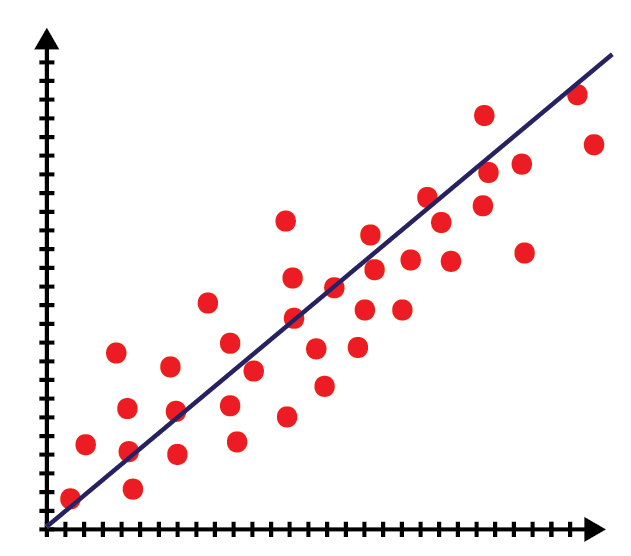
\includegraphics[width=3cm, height=3cm]{regression_chart}

\paragraph{Parameter estimations in the bivariate case}\mbox{} \\
\mbox{} \\
Generalizing the regression line equation, one can, in the case of the two-variable problem, start from:

$\hat{y} = mx + b +\varepsilon_{i}$,

Where:
\begin{itemize}
    \item $\hat{y}$ is the dependent (response) variable.
    \item $m$ is the line angular coefficient.
    \item $b$ is the line intercept.
    \item $\varepsilon_{i}$ is the statistical error.
\end{itemize}

At this point, the regression problem results in the determination of $m$ and $b$ so as to express the functional relationship between $y$ and $x$ as best as possible.

$\displaystyle m = \frac{n \sum{xy} - \sum{x}\sum{y}}{n\sum{x^2} - (\sum{x})^2}$ \\ \mbox{} \\
\mbox{} \\
$\displaystyle b = \frac{\sum{y} - m\sum{x}}{n}$

\clearpage
\section{Data Visualization}
Data visualization (data viz) is the graphical representation of data. 
The main goals of data visualization are to make the phenomena within the dataset more evident, convey the embedded information in the analysis more efficiently, and reinforce cognitive aspects of the provided study (e.g., ease of reporting, memorability).

While data visualization pertains to the field of science and statistics, it has also taken on cross-cutting significance in purely artistic or design-related contexts.

Data visualization  is so relevant that it could be considered a discipline within a discipline, with a deep vertical of study and insight that spans mathematical, scientific, statistical, cognitive, and humanistic domains. 

The recent spread of data science has made data viz even more important.

However, this paper will be limited to exploring some of the best-known forms of graphical representation in the field of statistics, and some of their properties.

\subsection{Scatter Plot}
A scatter plot is a type of plot or mathematical diagram using Cartesian coordinates to display values for typically two variables for a set of data. Every data point is displayed as a dot.

Scatter plot has its most significance with continuous distributions. 

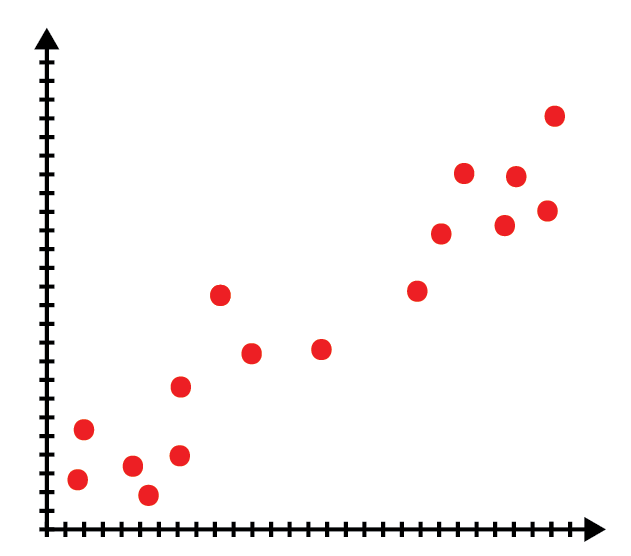
\includegraphics[width=3cm, height=3cm]{plot_chart}

\subsection{Line Chart}
Line charts show the evolution of a continuous variable (often over a time horizon).
A line chart is a way of plotting data points on a line. 
It is used to show trend data, or the comparison of two data sets.

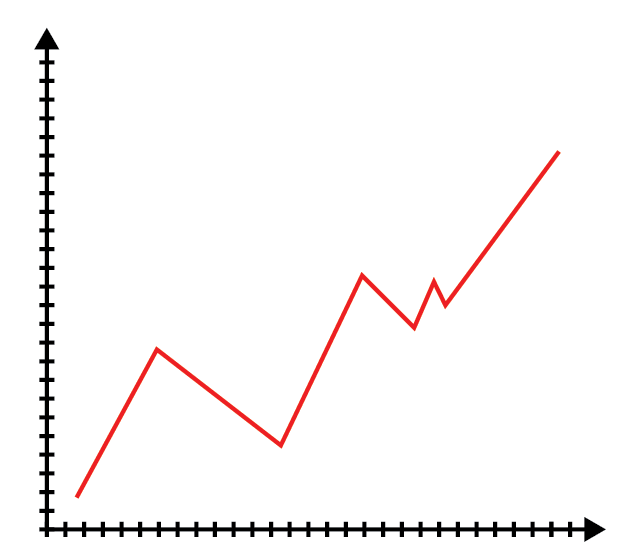
\includegraphics[width=3cm, height=3cm]{line_chart}

\subsection{Dot Plot}\footnote{In some texts, also called Line Plot.}
Dot plot is a way to display data frequency piled over data points and along a number line. 

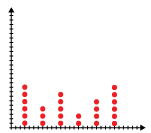
\includegraphics[width=3cm, height=3cm]{dot_plot}

\subsection{Histograms}
A histogram is a bar chart that groups continuous data into ranges. Ranges are discretional to the creator of the chart. For example, overall user ages (continuous dataset) can be grouped in clusters such as 0-10, 10-20 and such.

Histogram bars are adjacent (no spaces between bars).

Histograms don’t have to be confused with bar charts:
\begin{itemize}
    \item Histograms visualize quantitative data or numerical data. Usually, histograms display continuous variables. 
    \item Bar charts display categorical (discrete) variables. 
\end{itemize}

Correctly labeling horizontal ($X$) axis of an histogram chart is important in order to make it readable.

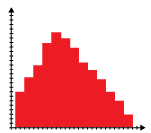
\includegraphics[width=3cm, height=3cm]{histogram_chart}

\subsection{Bar Plot}
Bar plots are usually used to display categorical data along the horizontal axis. That is, discrete data such as products, countries, car types and such. 

Bar within a bar chart are not adjacent. Data on the bar plots are often ordered, in order to enhance chart comprehension. 

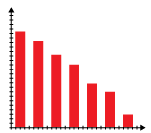
\includegraphics[width=3cm, height=3cm]{bar_chart}

\subsection{Ogive}
An ogive (oh-jive), sometimes called a cumulative frequency chart, is a type of frequency chart that shows cumulative frequencies. In other words, the cumulative percentages are added on the graph from left to right.

An ogive graph plots cumulative frequency on the y-axis and class boundaries along the x-axis. It’s very similar to a histogram, only instead of rectangles, an ogive has a single point marking where the top right of the rectangle would be. 

It is usually easier to create this kind of graph from a frequency table

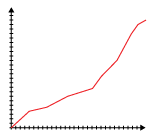
\includegraphics[width=3cm, height=3cm]{ogive_chart}

\subsection{Box and Whisker Plot}
A box and whisker plot is defined as a graphical method of displaying variation in a set of data. It is usually used to display data according to quartile intervals.

BWP are also called: box plot, box and whisker diagram, box and whisker plot with outliers\footnote{"Diagramma a scatola e baffi in italiano"}.

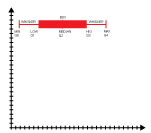
\includegraphics[width=4cm, height=4cm]{box_whisker_chart}

\paragraph{Box and whisker vs candlestick chart}\mbox{} \\
\mbox{} \\
Mathematically speaking there is no difference. Both show an upper and lower boundary and points outside these boundaries. However:
A candlestick chart is mainly used in the finance industry. Its most popular application is to show share price. It is mainly used in the vertical position.

A  box and whisker chart tends to be used in non-finance industries. For example, the level of sales of various stores or inventory levels etc. The box and whisker can be shown horizontally as well as vertically. They are often found with labels showing various statistical informations. 

\subsection{Violin Plot}
A violin plot is a method of plotting numeric data. It is similar to a box plot, with the addition of a rotated kernel density plot on each side.

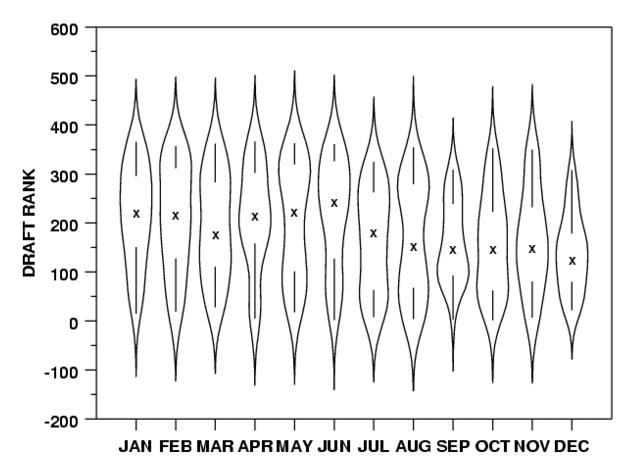
\includegraphics[width=5cm, height=3cm]{violin_chart}

\subsection{KDE Plot}

KDE Plot described as Kernel Density Estimate is used for visualizing the Probability Density of a continuous variable. It depicts the probability density at different values in a continuous variable. We can also plot a single graph for multiple samples which helps in more efficient data visualization.
Kernel density estimates are closely related to histograms, but can be endowed with properties such as smoothness or continuity by using a suitable kernel.

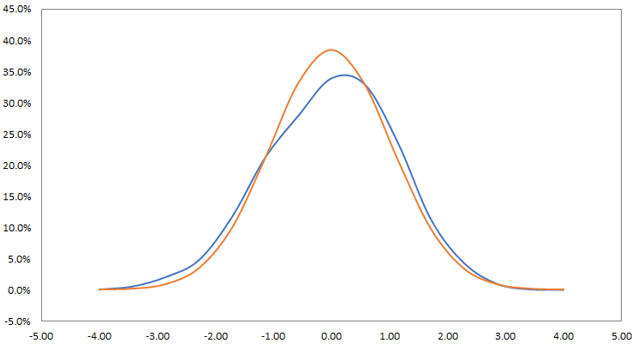
\includegraphics[width=5cm, height=3cm]{kde_chart}
\clearpage

\section{Combinatorics}
Combinatoric is an area of mathematics primarily concerned with counting, both as a means and an end in obtaining results, and certain properties of finite structures. It is closely related to many other areas of mathematics and has many applications ranging from logic to statistical physics and from evolutionary biology to computer science.

\subsection{Factorials}
In mathematics, the factorial of a non-negative integer $n$, denoted by $n!$, is the product of all positive integers less than or equal to $n$. The factorial of $n$ also equals the product of $n$ with the next smaller factorial.

5! = 5 * 4 * 3 * 2 * 1 = 120

An interesting property is also:

$n! = n * (n-1)!$

Example:
5! = 5 * 4! = 120

This leads to:
$\frac{n!}{(n-1)!} = \frac{n(n-1)!}{(n-1)!} = n$

\paragraph{Factorials and 0}\mbox{} \\
\mbox{} \\
Factorials deal only with natural numbers, hence 0 is omitted in the series (otherwise $n! = 0$).

But why 0! = 1 ?

It’s proven that:

$(n-1)! = \frac{n!}{n}$

This means that: \\
4! = 24 \\
3! = 24 / 4 = 6 \\
2! = 6 / 3 = 2 \\
1! = 2 / 2 = 1 \\
0! = 1 / 1 = 1 \\

And, following the same logic: \\
-1! = 1 / 0 = ND \\

that’s why $n!$ if $n \in {N} $ 

\subsection{Permutations}
A permutation of a set of objects is an arrangement of the objects \textbf{in a certain order}. 
Permutations differ from combinations, which are selections of some members of a set regardless of order. 

Usually permutations refer to all the possible arrangements (all the possible permutations of a set of objects). 

Permutations are calculated as factorials $(n!)$

Permutations are relevant when working with numbers, since "575" is not equal to "577" nor "557".

\subsection{Combinations}
A combination is a selection of items from a set that has distinct members, such that the order of selection does not matter (unlike permutations). 
For example, given three fruits, say an apple, an orange and a pear, there are three combinations of two that can be drawn from this set: 
\begin{itemize}
    \item an apple and a pear;
    \item an apple and an orange;
    \item a pear and an orange.
\end{itemize} 
Combinations \textbf{is an unordered selection} of objects from a set of objects.

More formally, a $k-combination$ of a set $S$ is a subset of $k$ distinct elements of $S$.

Combinations are relevant when working with products, or people: apple and orange is equal to orange and apple. A team with Mark and Tom is equal to a team with Tom and Mark.

The number of combinations from a set of $n$ objects taken $k$ a time is:

$\displaystyle C _n ^k = \binom{n}{k} = \frac{n!}{k!(n - k)!}$

\subsubsection{Permutations, Combinations and Dispositions}
\begin{center}
\begin{tabular}{|m{2cm}|c|c|}
\hline
& REPETITION & NO REPETITION (simple) \\ \hline
&&\\[-1em]
Permutations & $\displaystyle n^k$ & \makecell{$\displaystyle \frac{n!}{(n - k)!}$ \\[15pt] where $k = \text{cluster size}$ \\[15pt] $\displaystyle \frac{n!}{k1! * k2! * kn!}$ \\[15pt] where $k = \text{items repeated}$} \\[50pt] \hline
&&\\[-1em]
Combinations & $\displaystyle \frac{(n + k - 1)}{k!(n - 1)!}$ & $\displaystyle \frac{n!}{k!(n - k)!}$ \\[25pt] \hline
&&\\[-1em]
Dispositions & $\displaystyle n^k$ & $\displaystyle \frac{n!}{(n - k)!}$ \\[25pt] 
\hline
\end{tabular}
\end{center}

\paragraph{Examples}\mbox{} \\
\mbox{} \\
\textbf{Permutations with repetitions} \\ 
How many phone numbers of 7 digits can we generate using all the numbers from 0 to 9, allowing every specific case (such as "all zeros" being a valid number)?

$n = \text{[0, 1, 2, 3, 4, 5, 6, 7, 8, 9]} = 10$ \\
$k = \_ \_ \_ \_ \_ \_ \_ = 7$ \\ 
Each slot of k allows 10 combinations, so it’s $n^k = 10^7$

\textbf{Permutations with no repetitions example} \\
Find all the way the word MAMA can be arranged. 

n = 3 \\ 
k1 = 2 (the letter M is repeated 2 times) \\
k2 = 2 (the letter A is repeated 2 times) \\ 
4! / (2! * 2!) = 24 / 4 = 6 \mbox{} \\
\mbox{} \\
How can we arrange 5 students in 3 chairs? \\ 

n = 5 (all the students we have to pick from). \\
k = 3 (seats available). \\
5! / (5 - 3)! = 120 / 2 = 60 \mbox{} \\
\mbox{} \\

\paragraph{When to use permutations, combinations or dispositions? A diagram}\mbox{} \\
\mbox{} \\
Key insight: \\ 
Is the order relevant?
\begin{itemize}
    \item YES = PERMUTATIONS (ex. numbers)
    \item NO = COMBINATIONS (ex. people in teams)
\end{itemize}

\begin{adjustwidth}{-2.0cm}{-3.0cm}

    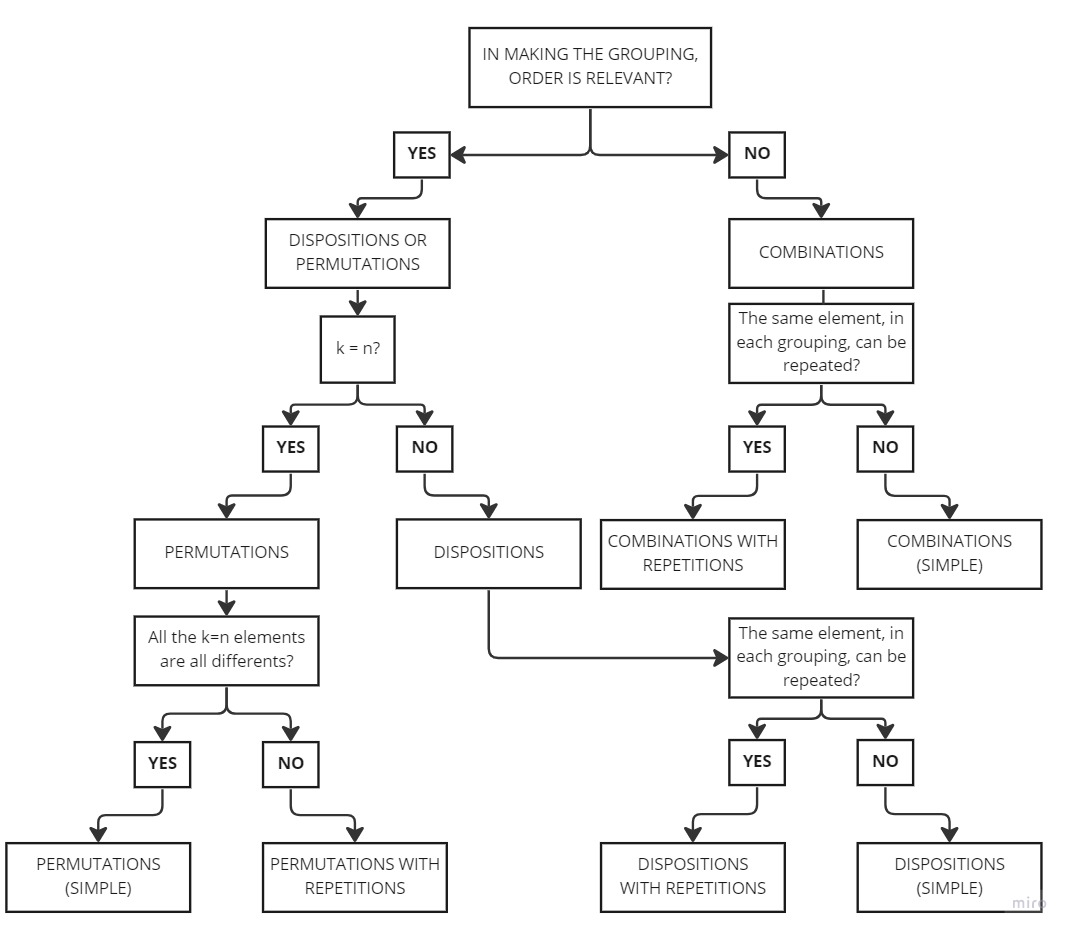
\includegraphics[width=20cm, height=20cm]{stat_diagram}

\end{adjustwidth}
\clearpage

\section{Probability}
Probability is the branch of mathematics that deals with how likely an event is to occur, or how likely is that a given proposition is true.

\paragraph{Probability Notation}\mbox{} \\

\begin{center}
\begin{tabular}{|c|c|c|}
\hline
$P(A)$ & Individual probability & The probability of event $A$ happening \\ \hline
&&\\[-1em]
$P(A')$ & Complement & The probability of event A not happening \\ \hline
&&\\[-1em]
$P(A')$ & Complement & The probability of event A not happening \\ \hline
&&\\[-1em]
$P(A \cup B)$ & Union & \makecell{The probability of both A and B happening for both datasets \\ (all elements of A plus all elements of B).} \\ \hline
&&\\[-1em]
$P(A \cap B)$ & Union & \makecell{The probability of both A and B happening for both datasets \\ (all elements of A plus all elements of B).} \\ \hline
&&\\[-1em]
$P(A | B)$ & Dependent & The probability of A given that B has occurred. \\
\hline
\end{tabular}
\end{center}

\mbox{} \\

\textbf{Example}\\ 
If $P = \{1,3,5,7,9\}$ and $Q = \{2,3,5,7\}$ \\
What are $P \cup Q$, and $P \cap  Q$? \\ 
\mbox{} \\
$P \cup Q = \{1,2,3,5,7,9\}$ \\ 
$P \cap Q = \{3,5,7\}$ \\

\subsection{Simple Probability}
Simple probability define how likely a specific event $A$ is going to happen in the given scenario. 

$P(A) = \text{target events / total events}$ \\
\mbox{} \\
And, consequentially: \\
\mbox{} \\
$P(A') = 1 - P(A)$

\paragraph{Experimental and Expected probability}\mbox{} \\
\mbox{} \\
\begin{itemize}
    \item Experimental probability is the probability resulting from empirical experimentations, such as flipping a coin 100 times and recording the results in a datasheet.
    \item Expected probability is the theoretical probability coming from applying the probability formula to the scenario.
\end{itemize}

The expected probability of having head over a coin toss is 50\%. However over a 100 tosses, the experimental probability may vary (ex. resulting in 30\% heads).

\paragraph{Law of Large Numbers}\mbox{} \\
\mbox{} \\
The law of large numbers, or Bernoulli's theorem (since its first formulation is due to Jakob Bernoulli), describes the behavior of the mean of a sequence of $n$ trials of a random variable, independent and characterized by the same probability distribution (n measurements of the same magnitude, $n$ tosses of the same coin, etc.), as the numerosity of the sequence itself $n$ tends to infinity.

\subsubsection{Probability Addition Rule}
If A and B are two events in a probability experiment, then the probability that either one of the events will occur is: \\ 
\mbox{} \\
P(A or B) = P(A)+P(B) − P(A and B) \\ 
\mbox{} \\
Or, with sets notation as: \\ 
\mbox{} \\
$P(A \cup B) = P(A)+P(B)−P(A \cap B)$ 

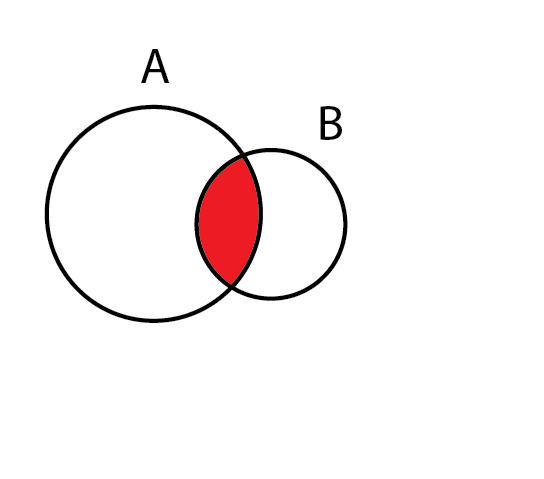
\includegraphics[width=3.5cm, height=3cm]{intersection}

If A and B are two mutually exclusive events, \\ 
$P(A \cap B) = 0$. Then the probability that either one of the events will occur is: \\
\mbox{} \\
$P(A or B)=P(A)+P(B)$ \\
\mbox{} \\
Or, with sets notation as: \\ 
\mbox{} \\
$P(A \cup B)=P(A) + P(B)$ \\ 

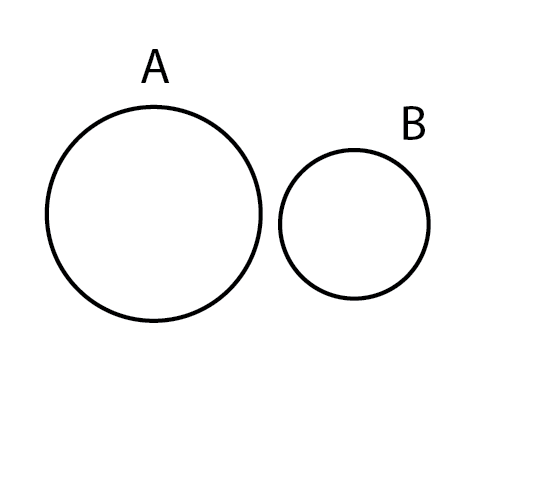
\includegraphics[width=3.5cm, height=3cm]{independent}

\textbf{Fundamental rule for addition or product in probability calculation} \\

\begin{itemize}
    \item Given two \textbf{independent} events, the probability of them \textbf{occurring both} is given by the \textbf{product} of the individual probabilities. 
    \begin{itemize}
        \item Example: having a head out of two coin flips.
    \end{itemize}
    \item The probability of two or more \textbf{alternative} events occurring is equal to the \textbf{sum} of the individual probabilities. 
    \begin{itemize}
        \item Example: having 1 or 2 out of a dice roll.
    \end{itemize}
\end{itemize}

\subsubsection{Conditional Probability for Independent and Dependent Events}
\textbf{Independent event probability} \\ 
The probability of A and B happening. \\
\mbox{} \\
$P(A \cap B) = P(A) * P(B)$ \\ 
\mbox{} \\
Tossing two coins $A$ and $B$, what is the probability of having two head values? \\ 
Coins are independent each other, so: \\ 
\mbox{} \\
$P(A \cap B) = 1 / 2 * 1 / 2 = 1 / 4 $ \\ 
\mbox{} \\
Defective rate in a production line is 2\%. \\ 
What is the probability of having 3 defective products in a row?\\
\mbox{} \\
$P(A \cap B \cap  C) = 2 / 100 * 2 / 100 * 2 / 100 = \frac{8}{100^3} = 1 / \text{125'000}$ \\ 
\mbox{} \\
\textbf{Dependent event probability}
\mbox{} \\
The probability of A and B, given that A has already occurred. \\ 
\mbox{} \\
$P(A \cap B) = P(A) * P(B | A)$ \\ 
\mbox{} \\
What’s the probability of drafting two Kings in a row from a standard deck of cards? \\

$P(A \cap B) = 4 / 52 * 3 / 51  = 1 / 13 * 1 / 17 = 1 / 221$

\textbf{Reminder}

If $P(B) = P(B | A)$ then the events must be independent.

\subsection{Bayes Theorem}
Bayes' theorem describes the probability of an event, based on prior knowledge of conditions that might be related to the event. 

$\displaystyle P(A\mid B)={\frac {P(B\mid A)P(A)}{P(B)}}$ \\ 

Where: 
\begin{itemize}
    \item $A$ and $B$ are events and $P(B) \neq 0 $.
    \item $P(A)$ is the probability of event $A$.
    \item $P(B)$ is the probability of event $B$.
    \item $P(A | B)$ is the probability of observing event $A$ if $B$ is true.
    \item $P(B | A)$ is the probability of observing event $B$ if $A$ is true.
\end{itemize}

\paragraph{Example 1.}\mbox{} \\
\mbox{} \\
We have two assembly lines, 1 and 2. \\ 
Line 1 has a defective rate of 3\%, Line 2 of 1\%. \\ 
Given a defective part, what is the probability that it came from line 1? \\ 
\mbox{} \\
Let’s call:
\begin{itemize}
    \item $P(B)$ the probability of a product being defective.
    \item $P(A)$ the probability of a product coming from line 1.
\end{itemize}
Hence: \\ 
\mbox{} \\
$P(A) = 1 / 2$ \\  
(with the available data, we must assume we have a 50\% likelihood from two lines). 

$P(B | A)$ = probability of $B$(defect) if $A$(product is coming from line 1) has occurred = $3 / 100$ (this is the info provided by the context already).

$P(B)$ = overall probability of having a defective product = $[(1 / 2) * (3 / 100)] + [(1 / 2) * (1 / 100)] =   3 / 200 + 1/ 200 = 4 / 200 = 1 / 50$

Applying Bayes Theorem, then:

$P(A | B) = [(3 / 100) * (1 / 2)] / (1 / 50) = (3 / 200) / (1 / 50) = (3 / 200) * (50 / 1) = 150 / 200 = 3 / 4 = 75\% $

\paragraph{Example 2.}\mbox{} \\
\mbox{} \\
You’re tested for a disease that occurs 1 out of 1’000 people. \\ 
Test accuracy is 99\%. \\ 
You are tested positive. \\ 
What is the change you actually have the disease? \\ 
\mbox{} \\
\begin{itemize}
    \item Population: $\text{1'000}$
    \item Incidence: $(1/\text{1’000}) = \text{0.001}$
    \item Accuracy: 99\%
    \item False positive \ negative: $(100\% - 99\%) = 1\%$
\end{itemize}

\begin{center}
\begin{tabular}{|c|c|c|c|}
\hline
 & SICK & NOT SICK & TOTAL \\ \hline
&&&\\[-1em]
TESTED POS & 0.99[1] & 9.99[3] & 10.98 \\ \hline
&&&\\[-1em]
TESTED NEG & 0.01[2] & 989.01[4] & 989.02 \\ \hline
&&&\\[-1em]
TOTAL & 1 & 999 & 1'000 \\ 
\hline
\end{tabular}
\end{center}

\mbox{} \\  

{[1]} = $\text{1’000} * 0.001 * 99\%$ \\ 
{[2]} = $\text{1’000} * 0.001 * 1\%$ \\ 
{[3]} = $(\text{1’000} * (1 - 0.001)) * 1\%$ \\ 
{[4]} = $(\text{1’000} * (1 - 0.001)) * 99\%$ \\

\mbox{} \\

$P(A)$ = probability of being sick = $0.001$ \\ 
$P(B)$ = probability of having a positive test = $10.98 / \text{1’000}$ \\ 
$P(B|A)$ = probability of having a positive test being sick = $0.99$ \\ 
$P(A|B)$ = probability of being sick having a positive test = $10.98 / 0.99$ (or applying Bayesian formula) = $9\%$ \\ 

\subsubsection{Tree Diagrams}
A tree diagram is a type of diagram that can be useful as an aid in computing probabilities. \\ 
For example, consider an experiment of tossing a six-sided die. Each
time the experiment is repeated, the probability of obtaining a 1 (event ) is $P(A) = 1 / 6$. 
If you are only concerned with whether the number is 1 or not 1, and the experiment is repeated three times, then eight different sequences of events are possible. \\ 
The tree diagram below shows the probabilities of these eight sequences of events.

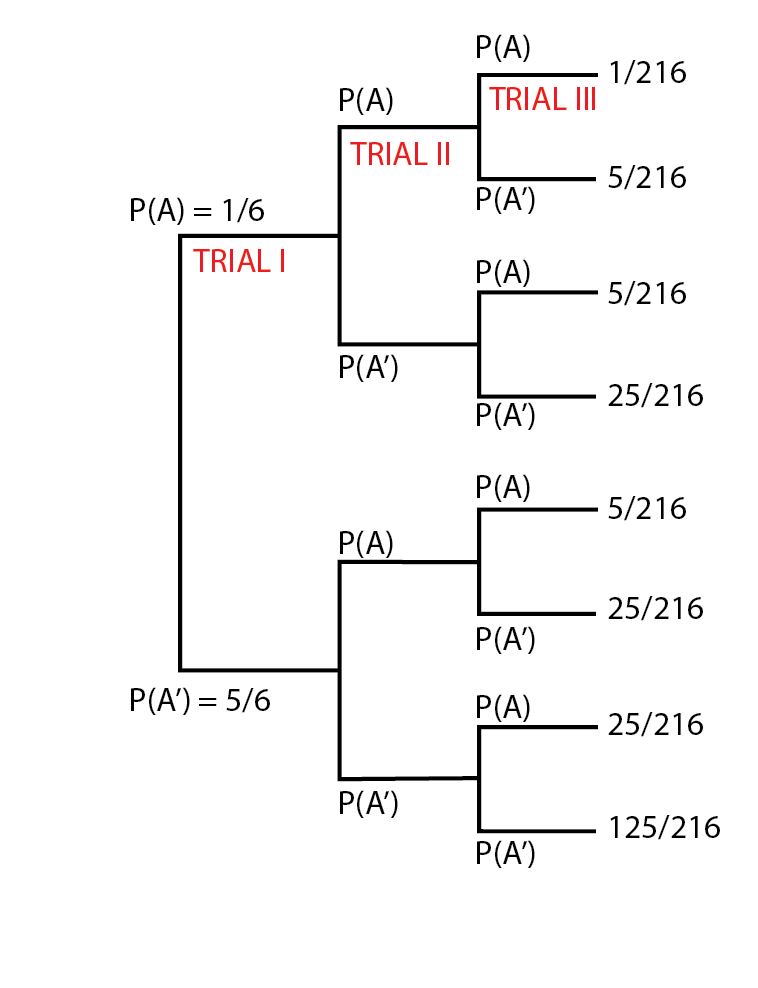
\includegraphics[width=5cm, height=7cm]{tree_diagram}

\subsection{Discrete Probability}
Discrete probability deals with events with a finite or countable number of occurrences. \\ 
This is in contrast to a continuous distribution, where outcomes can fall anywhere on a continuum. 

Common examples of discrete distribution include the binomial, Poisson, and Bernoulli distributions.

\textbf{Example of of discrete probability}
What is the probability of having head out of 3 coin flips?
\begin{itemize}
    \item Number of variable: 2 (head or tail).
    \item Number of events: 3 flips.
    \item Total number of combinations: $2^3 = 8$
\end{itemize}

Possible outcomes: \\ 
\begin{center}
\begin{tabular}{|c|c|}
\hline
EVENT & N. OF HEADS \\ \hline
&\\[-1em]
HHH & 3 \\ \hline
&\\[-1em]
THH & 2 \\ \hline
&\\[-1em]
HTH & 2 \\ \hline
&\\[-1em]
TTH & 1 \\ \hline
&\\[-1em]
HHT & 1 \\ \hline
&\\[-1em]
THT & 1 \\ \hline
&\\[-1em]
HTT & 1 \\ \hline
&\\[-1em]
TTT & 0 \\
\hline
\end{tabular}
\end{center}

\begin{center}
\begin{tabular}{|c|c|}
\hline
\makecell {HEADS IN 3 \\ COIN FLIPS (X)} & P(X)\\ \hline
&\\[-1em]
0 & 1/8 \\ \hline
&\\[-1em]
1 & 3/8 \\ \hline
&\\[-1em]
2 & 3/8 \\ \hline
&\\[-1em]
3 & 1/8 \\ 
\hline
\end{tabular}
\end{center}

$P(X) = 0 * 1/8 + 1 * 3/8 + 2 * 3/8  + 3 * 1/8 = 12 / 8  = 3 / 2 = 150\%  $ \\ 
\mbox{}\\
Mean = $3 / 2$ \\ 
\mbox{}\\
Variance = $\sigma^2 = (0 - 3/2)^2 * 1/8 + (1 - 3/2)^2 * 3/8 + (2 - 3/2)^2 * 3/8 + (3 - 3/2)^2 * 1/8 =  0,75$ \\ 
\mbox{}\\
Standard Deviation = $\sigma = \sqrt{\sigma^2} = 0.866$ \\ 
\mbox{}\\
Note that in practical terms, a rational number is not making sense in a discrete probability calculation (we can’t have half of a coin flip or 1.5 heads as a result. This is a case of theoretical probability vs experimental probability).   

\subsubsection{Transforming Random Variables}
How the distribution of a random variable changes when the variable is transformed in a deterministic way?

\paragraph{Shifting Data}\mbox{} \\
\mbox{} \\
Shifthing data means adding a constant $k \in \mathbb{R}$ to each member of a dataset.
\begin{center}
\begin{tabular}{|c|c|}
\hline
X & Y\\ \hline
&\\[-1em]
3 & 3 + K \\ \hline
&\\[-1em]
3 & 3 + K \\ \hline
&\\[-1em]
7 & 7 + K \\ \hline
&\\[-1em]
10 & 10 + K \\ \hline
&\\[-1em]
12 & 12 + K \\ 
\hline
\end{tabular}
\end{center}

\begin{center}
\begin{tabular}{|c|c|}
\hline
Dataset & Shifted, K\\ \hline
&\\[-1em]
Mean: 6 & Mean: 6 + K \\ \hline
&\\[-1em]
Median:  & Median: 3 + K \\ \hline
&\\[-1em]
Mode: 3 & Mode: 3 + K  \\ \hline
&\\[-1em]
Range: 10 & Range: 10 \\ \hline
&\\[-1em]
IQR: 8 & IQR: 8 \\ \hline
&\\[-1em]
St. Dev: $\sigma$ & St. Dev: $\sigma$ \\ 
\hline
\end{tabular}
\end{center}
\textbf{Impact of K-shifting:} while mean, median and mode will change of a K-addictive factor, range, IQR and standard deviation will stay the same since in fact the shape (and, more precisely, the distance between each datapoint) will not change.

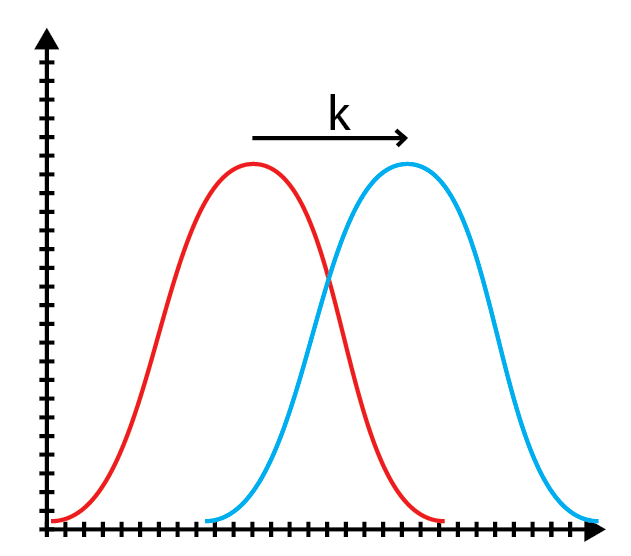
\includegraphics[width=3cm, height=3cm]{shifted}

\paragraph{Scaling Data}\mbox{} \\
\mbox{} \\
Scaling data means multipying each member of a dataset by a constant $k$.
\begin{center}
\begin{tabular}{|c|c|}
\hline
Dataset & Scaled, K\\ \hline
&\\[-1em]
Mean: 6 & Mean: 6K \\ \hline
&\\[-1em]
Median:  & Median: 3K \\ \hline
&\\[-1em]
Mode: 3 & Mode: 3K  \\ \hline
&\\[-1em]
Range: 10 & Range: 10K \\ \hline
&\\[-1em]
IQR: 8 & IQR: 8K \\ \hline
&\\[-1em]
St. Dev: $\sigma$ & St. Dev: $\sigma$ K \\
\hline
\end{tabular}
\end{center}
\textbf{Impact of K-scaling:} all the values are impacted by a k-magnitude factor.
Consider that both assumptions will be valid in a mixed case such as: 
$N(X) = 10x$ - 2 ($*x$ - 2 applies for mean, median and mode, while only $*x$ applies to standard deviation, IQR and range).

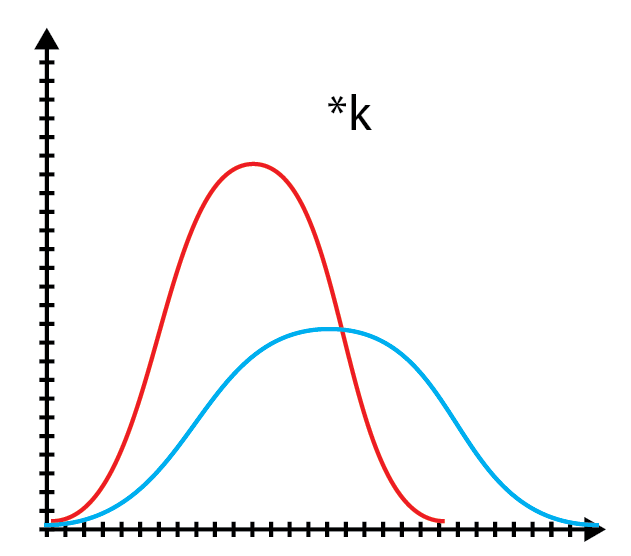
\includegraphics[width=3cm, height=3cm]{scaled}

\subsubsection{Linear Combinations of Random Variables}
Let $X_1$ and $X_2$ be two independent random variables. Let $a$ and $b$ be scalars. Then a linear combination of the variables $X_1$ and $X_2$ and is defined to be any other random variable of the form $Y= aX_1 + bX_2$. 

Base assumptions:
\begin{itemize}
    \item Variables must be independent.
    \item Variables must have matching units of measurements.
\end{itemize}

\begin{center}
\begin{tabular}{|c|c|c|}
\hline
 & $\sum$ & $\Delta$  \\ \hline
&&\\[-1em]
Combination & $\sum = X + Y $ & $\Delta = X - Y$ \\ \hline
&&\\[-1em]
Mean & $\mu = \mu x + \mu y $ & $\mu = \mu x - \mu y$ \\ \hline
&&\\[-1em]
Variance & $\sigma^2 = \sigma^2 x + \sigma^2 y$ & $\sigma^2 = \sigma^2 x + \sigma^2 y$ \\
\hline
\end{tabular}
\end{center}

\textbf{Example:}
Time in hours 4 managers manage timesheets: \\ 
X = [1, 2, 2, 3] \\ 
\mbox{} \\
Time in hours 4 HRs manages payrolls on such timesheets: \\ 
Y = [2, 3, 5, 6] \\ 
\mbox{} \\

$\mu X$ = (1 + 2 + 2 + 3) / 4 = 2 \\
\mbox{} \\
$\mu Y$ = (2 + 3 + 5 + 6) / 4 = 4 \\ 
\mbox{} \\
$\sigma^2 X$ = $[(1 - 2)^2 + (2 - 2)^2 + (2 - 2)^2 + (3 - 2)^2 ]$ / 4 = 0.5  \\
\mbox{} \\
$\sigma X$ =  $\sqrt{0.5}$ = 0.70 \\ 
\mbox{} \\
$\sigma^2 Y$ = $[(2 - 4)^2 + (3 - 4)^2 + (5 - 4)^2 + (6 - 4)^2]$ / 4 = 2.5  \\
\mbox{} \\
$\sigma Y$ =  $\sqrt{2.5}$ = 1.58 \\
\mbox{} \\
$X + Y$ \\
$\mu$ = 2 + 4 = 6 \\
\mbox{} \\
$\sigma^2$ = 0.5 + 2.5 = 3 \\ 
\mbox{} \\
$\sigma$ = $\sqrt{3}$ = 1.73 \\ 
\mbox{} \\
$X - Y$ \\ 
$\mu$ = $|$2 - 4$|$ = 2 \\ 
\mbox{} \\
$\sigma^2$ = 0.5 + 2.5 = 3 \\ 
\mbox{} \\
$\sigma$ = $\sqrt{3}$ = 1.73 \\

\subsubsection{Fair Game}
A fair game\footnote{Italian translation: gioco equo} is a game (a bet, as an example, or a lottery) in which the cost of playing the game equals the expected winnings of the game, so that net value of the game equals zero.

$W = B/p = 1$ 
\mbox{} \\
Where:
$W$ = win
$B$ = Bet
$p$ = probability

\textbf{Is state lottery a fair game?}\\ 
The Italian national lottery (“Lotto”) is a bingo where 5 numbers are drawn out of a poll of 90. Repetition is not allowed (extracted numbers are discarded)\footnote{\url{https://www.lotto-italia.it/lotto/come-dove-giocare/il-gioco/premi-del-lotto}}. 

Players win if they have all the 5 numbers on the card, in no specific order (there are also some minor prizes such as “ambo” for two numbers, “terno” for three numbers, and such. But the logic is the same).

A five is paying 6’000’000 times the bet.

It this fair? Intuitively, it’s not. 

But we are here not to assume but to investigate.

All the combinations\footnote{see Combinatorics chapter for details} of 5 numbers are $ \displaystyle C _n ^k = \binom{n}{k}$ hence:

$\frac{90!}{5!(90 - 5)!}$ = 43’949’268 

This is obviously matching the official lottery statement.

The probability of winning is then 1/43’949’268 = 0.00000228\%

Fair game will assume: 

$W = B/p = 1$

But we have:
W = 6’000’000
B = 1
p = 0.00000228\%

$W = B/p$ = 1 / 0.00000228\% = 43’949’268

How unfair is that game?

43’949’268 / 6’000’000 = 7.32

The Italian lotto is more than 7 times unfair for the player.
\clearpage

\section{Joint Distributions}
Joint distributions allow us to mathematically quantify the relationship between two distributions of data. 

Given two random variables that are defined on the same probability space, the joint probability distribution is the corresponding probability distribution on all possible pairs of outputs. 

The joint distribution can just as well be considered for any given number of random variables. 

The joint distribution encodes the marginal distributions, i.e. the distributions of each of the individual random variables. It also encodes the conditional probability distributions, which deal with how the outputs of one random variable are distributed when given information on the outputs of the other random variable(s).

\subsection{Covariance}
Covariance is a numerical value that provides a measure of how much two variables vary together.

It evaluates how the variables change together, providing the \textbf{direction} of the variation. 
It’s a measure of the variance between two variables. However, the metric does not assess the dependency between variables.

A \textbf{positive covariance} means that it’s expected both variables have a concordant behavior ($X$ grows, $Y$ grows, $X$ decreases, $Y$ decreases).

A \textbf{negative covariance} means that it’s expected both variables have a discordant behavior 
($X$ grows, $Y$ decreases, $X$ decreases, $Y$ grows).

A \textbf{neutral covariance} means that the variables have no relations with each other.

Expressed in mathematical notation, covariance formulas are:

\textbf{Population Covariance}: \\ 
$\displaystyle cov(x, y) = \frac{1}{n}\sum \limits_{i=1}^n (x_i - \bar{x})(y_i - \bar{y})$

\textbf{Sample Covariance}: \\ 
$\displaystyle cov(X, Y) = \frac{1}{N-1}\sum \limits_{i=1}^N (X_i - \bar{X})(Y_i - \bar{Y})$

\subsection{Correlation}
Correlation is a metric used to measure the \textbf{strength} of a  statistical relationship between two random variables. It’s also called a \textbf{measure} of relationship.

The correlation coefficient is a dimensionless metric and its value ranges from -1 to +1. 

The closer it is to +1 or -1, the more closely the two variables are related. 
If there is no relationship at all between two variables, then the correlation coefficient will be close to 0. 

However, if it is 0 then we can only say that there is no linear relationship. There could exist other functional relationships between the variables.

\begin{itemize}
    \item +1: positive correlation ($X$ grows, $Y$ grows, $X$ decreases, $Y$ decreases).
    \item -1: negative correlation ($X$ grows, $Y$ decreases, $X$ decreases, $Y$ grows).
\end{itemize}

While Covariance measures just the direction of variation between two variables, Correlation explores the strength and relation of the variation, in a standardized and comparable format.

In statistics application, there are three kind of correlation being applied:

\begin{itemize}
    \item Pearson (Parametric method).
    \item Spearman (Nonparametric method).
    \item Kendall (Nonparametric method).
\end{itemize}

\subsubsection{Pearson Correlation}
Pearson correlation is the most widely used correlation statistic to measure the degree of the relationship between linearly related variables. 

For the Pearson correlation, both variables should be normally distributed (normally distributed variables have a bell-shaped curve). 

Pearson correlation assumptions:
\begin{itemize}
    \item Each observation should have a pair of values.
    \item Each variable should be continuous.
    \item Data have no outliers.
    \item Variables linearity.
    \item Variables homoscedasticity (homogeneity of variance).
\end{itemize}

\textbf{For a population}\\
Pearson correlation is expressed with the greek letter $\rho$ (rho) when referred to population.
Given a pair of random variables $(X,Y)$, the formula for $\rho$is:

$\displaystyle \rho _{X,Y}={\frac{cov(X,Y)}{\sigma _{X}\sigma _{Y}}}$

where:
\begin{itemize}
    \item $\displaystyle {cov}$ is the covariance.
    \item $\displaystyle \sigma _{X}$ is the standard deviation of $X$.
    \item $\displaystyle \sigma _{Y}$  is the standard deviation of $Y$.
\end{itemize}

\textbf{For a sample}\\
Pearson's correlation coefficient, when applied to a sample, is commonly represented by $r_{xy}$ and may be referred to as the sample correlation coefficient or the sample Pearson correlation coefficient. 
We can obtain a formula for $r_{xy}$ by substituting estimates of the covariances and variances based on a sample into the formula above. 
Given paired data $\displaystyle \{(x_{1},y_{1}),\ldots ,(x_{n},y_{n})\}$ consisting of $n$ pairs, $r_{xy}$ is defined as:

$\displaystyle r_{xy}={\frac {\sum _{i=1}^{n}(x_{i}-{\bar {x}})(y_{i}-{\bar {y}})}{{\sqrt {\sum _{i=1}^{n}(x_{i}-{\bar {x}})^{2}}}{\sqrt {\sum _{i=1}^{n}(y_{i}-{\bar {y}})^{2}}}}}$

where:
\begin{itemize}
    \item $n$ is sample size.
    \item $x_{i},y_{i}$ are the individual sample points indexed with $i$.
    \item ${\textstyle {\bar {x}}={\frac {1}{n}}\sum _{i=1}^{n}x_{i}}$ (the sample mean); and analogously for $\bar {y}$.
\end{itemize}

Rearranging gives us this formula for $\displaystyle r_{xy}$:

${\displaystyle r_{xy}={\frac {n\sum x_{i}y_{i}-\sum x_{i}\sum y_{i}}{{\sqrt {n\sum x_{i}^{2}-\left(\sum x_{i}\right)^{2}}}~{\sqrt {n\sum y_{i}^{2}-\left(\sum y_{i}\right)^{2}}}}}}$

where $n,x_{i},y_{i}$ are defined as above.

This formula suggests a convenient single-pass algorithm for calculating sample correlations.

\subsubsection{Kendall Rank Correlation}
Kendall rank correlation is a non-parametric test that measures the strength of dependence between two quantitative or qualitative ordinal statistical variables. 

Kendall rank correlation is expressed with greek letter $\tau$ (tau)

$\displaystyle \tau = \frac{n_c - n_d}{n_c + n_d} = \frac{n_c - n_d}{n(n - 1)/2}$

where:
\begin{itemize}
    \item $n_c$ is the number of concordant pairs.
    \item $n_d$ is the number of discordant pairs.
    \item $n$ is the number of pairs.
\end{itemize}

Kendall rank assumptions:
\begin{itemize}
    \item Pairs of observations are independent.
    \item Two variables should be measured on an ordinal, interval or ratio scale.
    \item Monotonic relationship between the two variables.
\end{itemize}

\subsubsection{Spearman Rank Correlation}
Spearman rank is a non parametric measure of rank correlation (measure of statistical dependence between the rankings of two variables). Spearman rank is also defined as the Pearson correlation between the rank variables.

Spearman rank is denoted with same greeks as Pearson, $\rho$ and $r$.

For a sample of size $n$, the $n$ raw scores $ X_{i},Y_{i}$ are converted to ranks ${R} ({X_{i}}), {R} ({Y_{i}})$, and $ r_{s}$ is computed as:

$\displaystyle r_{s}=\rho _{{R} (X), {R} (Y)}={\frac { {cov} ( {R} (X),{R} (Y))}{\sigma _{ {R} (X)}\sigma _{{R} (Y)}}}$

where:
\begin{itemize}
    \item $\rho$ denotes the usual Pearson correlation coefficient, but applied to the rank variables.
    \item ${cov} ( {R} (X),{R} (Y))$  is the covariance of the rank variables.
    \item $\sigma _{ {R} (X)}, \sigma _{{R} (Y)}$ are the standard deviations of the rank variables.
\end{itemize}

\mbox{}\\

Spearman rank assumptions:
\begin{itemize}
    \item Pairs of observations are independent.
    \item Two variables should be measured on an ordinal, interval or ratio scale.
    \item Monotonic relationship between the two variables.
\end{itemize}

\subsubsection{Point-biserial Correlation coefficient}
The Point-Biserial correlation coefficient is used when one of the given variable is dichotomous (such as “head or tail” on a coin flip).

Point-biserial correlation coefficient is expressed with $r_{pb}$.

\clearpage

\section{Data Distributions}
In statistics, and specifically to the field of descriptive statistics, a distribution is a representation of how different modes of a character are distributed across the statistical units that make up the collective under study.

\subsection{Probability Mass Function (PMF)}
Probability mass function is a function that gives the probability that a discrete random variable is exactly equal to some value. 

$f(x) = P[X = x]$

where $X$ is the \textbf{discrete random variable} and $x$ is the \textbf{target value}.

\textbf{Example}:\\ 

What is the probability of picking a specific ball out of a jar with 100 balls, all the balls being equal? 
It’s 1/100, or 1\%.

\paragraph{PMF Visualization}\mbox{} \\
\mbox{} \\

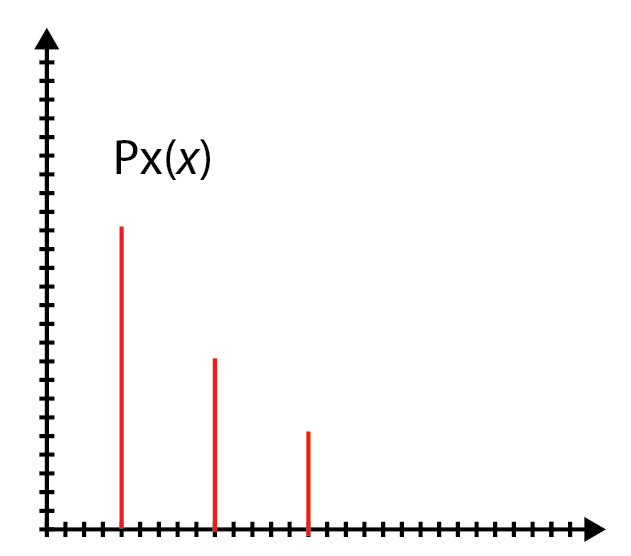
\includegraphics[width=3cm, height=3cm]{pmf}

\textbf{Discrete Uniform Distribution} \\ 
Discrete uniform distribution refers to discrete events where all the events have an equal chance of occurring (such as dice rolls).

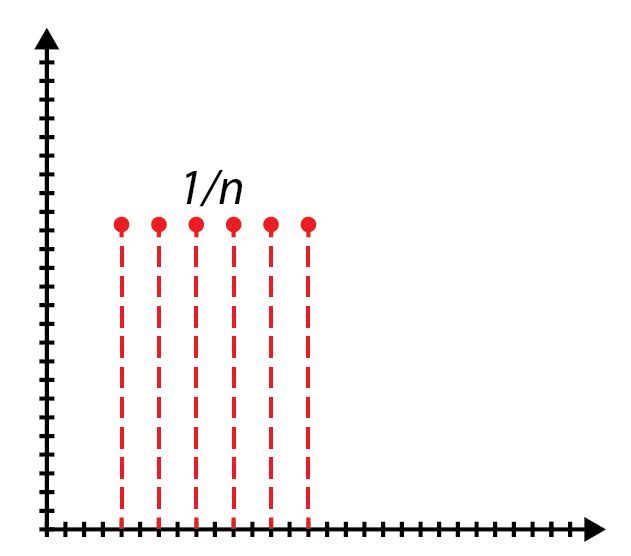
\includegraphics[width=3cm, height=3cm]{dud}

\paragraph{PMF Overview}\mbox{} \\

\begin{itemize}
    \item Notation: $\displaystyle {\mathcal{U}}\{a,b\}$ or $\displaystyle \text{unif} \{a,b\}$
    \item Parameters: $\displaystyle a,b$ integers with $\displaystyle b\geq a$, $\displaystyle n=b-a+1$
    \item Support: $\displaystyle k\in \{a,a+1,\dots ,b-1,b\}$
    \item PMF: $\displaystyle {\frac {1}{n}}$
    \item CDF: $\displaystyle {\frac {\lfloor k\rfloor -a+1}{n}}$ 
    \item Mean: $\displaystyle {\frac {a+b}{2}}$ 
    \item Median: $\displaystyle {\frac {a+b}{2}}$
    \item Mode:	N/A
    \item Variance: $\displaystyle {\frac {n^{2}-1}{12}}$
\end{itemize}

\subsection{Probability Density Function (PDF)}

In probability theory, a probability density function (PDF), or density of a \textbf{continuous random variable}, is a function whose value at any given sample (or point) in the sample space (the set of possible values taken by the random variable) can be interpreted as providing a relative likelihood that the value of the random variable would be close to that sample.

Density functions require switching from exact outcomes (such as for discrete variables) to approximations or interval ranges for an infinite set of values within the probability interval (in a continuous interval, the values of the variable are so small to be practically uncountable).

$\displaystyle Pr[a\leq X\leq b]=\int _{a}^{b}f_{X}(x)dx$

with:
\begin{itemize}
    \item $P(x=c)=0$
    
\end{itemize}

More technically, In a continuous distribution (e.g. continuous uniform, normal, and others), the probability is calculated by integration, as an area under the probability density function.

For $f(x)$ to be a legitimate PDF, it must satisfy the following two conditions:
\begin{itemize}
    \item $f(x) \geq 0$, $\forall x \in \mathbb{R}$
    \item $\displaystyle \int _{-\infty }^{\infty } f(x)dx=1$
\end{itemize}
If a random variable $X$ is given and its distribution admits a probability density function $f$, then the expected value of $X$ (if the expected value exists) can be calculated as:

$\displaystyle {E} [X]=\int _{-\infty }^{\infty }xf(x)dx$

Not every probability distribution has a density function: the distributions of discrete random variables do not, for example.

Note also that within a PDF, the probability of having a specific, exact value (such as in PMF) is always equal to zero. The expectation is for an approximation $(a < X < b)$ and not for an equality $(X = a)$.

There are many kinds of probability density functions (actually more than 100, going from very common normal distribution, Pareto distribution, uniform distribution, to other less common distributions such as Polya-Gamma). 

\paragraph{PDF Visualization}\mbox{} \\
\mbox{} \\

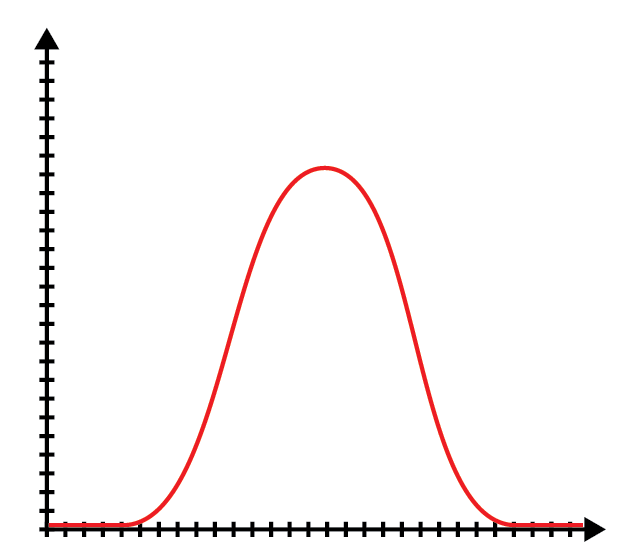
\includegraphics[width=3cm, height=3cm]{pdf}

\textbf{Continuous Uniform Distribution} \\
In probability theory and statistics, the continuous uniform distribution or rectangular distribution is a family of symmetric probability distributions. The distribution describes an experiment where there is an arbitrary outcome that lies between certain bounds. 

The bounds are defined by the parameters, a and b, which are the minimum and maximum values. The interval can either be closed (ex. [a, b]) or open (ex. (a, b)).
Therefore, the distribution is often abbreviated U (a, b), where U stands for uniform distribution.

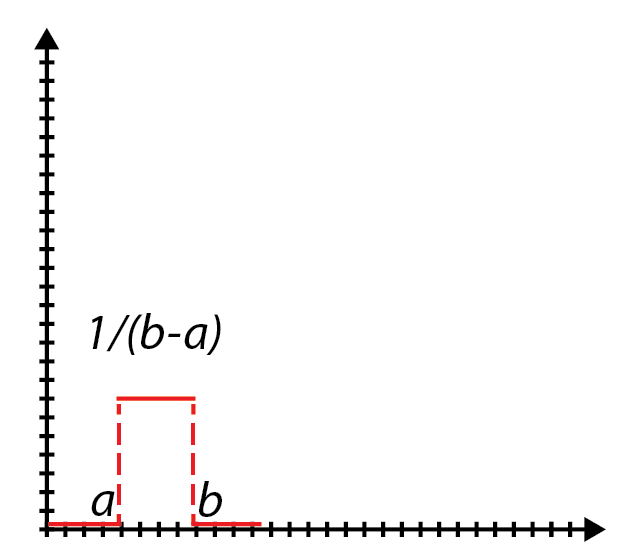
\includegraphics[width=3cm, height=3cm]{cud}

\paragraph{CUD Overview}\mbox{} \\

\begin{itemize}
    \item Notation: $\displaystyle {\mathcal {U}}_{[a,b]}$
    \item Parameters: $\displaystyle -\infty <a<b<\infty$
    \item Support: $\displaystyle x\in [a,b]$
    \item PDF: $\displaystyle {\begin{cases}{\frac {1}{b-a}}&{\text{for }}x\in [a,b]\\0&{\text{otherwise}}\end{cases}}$
    \item CDF: $\displaystyle {\begin{cases}0&{\text{for }}x<a\\{\frac {x-a}{b-a}}&{\text{for }}x\in [a,b]\\1&{\text{for }}x>b\end{cases}}$
    \item Mean: $\displaystyle {\tfrac {1}{2}}(a+b)$
    \item Median:	$\displaystyle {\tfrac {1}{2}}(a+b$)
    \item Mode:	any value in $\displaystyle (a,b)$
    \item Variance:	$\displaystyle {\tfrac {1}{12}}(b-a)^{2}$
\end{itemize}

\subsection{Cumulative Distribution Functions (CDF)}
The cumulative distribution function (CDF) is the probability that the variable takes a value less than or equal to x. 

$F(x) = P(X \leq x)$, $\forall x \in \mathbb{R}$  

CDF expresses the cumulative probability of a given event.

\textbf{Discrete Cumulative Distribution Function} \\
A CDF in a discrete set.

As an example, rolling a standard dice:
\begin{itemize}
    \item the CDF of having no numeric input is 0.
    \item the CDF of a number from 1 to 6 is 1 (6/6).
    \item the CDF of a number less or equal to 3 is 3/6.
\end{itemize}

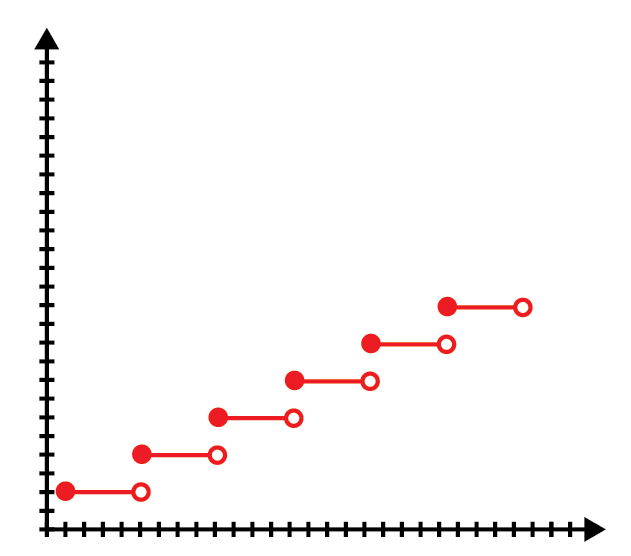
\includegraphics[width=3cm, height=3cm]{discrete_cdf}

\textbf{Continuous Cumulative Distribution Function} \\
The cumulative distribution function, CDF, or cumulant is a function derived from the probability density function for a continuous random variable. It gives the probability of finding the random variable at a value less than or equal to a given cutoff. Many questions and computations about probability distribution functions are convenient to rephrase or perform in terms of CDFs, ex. computing the PDF of a function of a random variable.

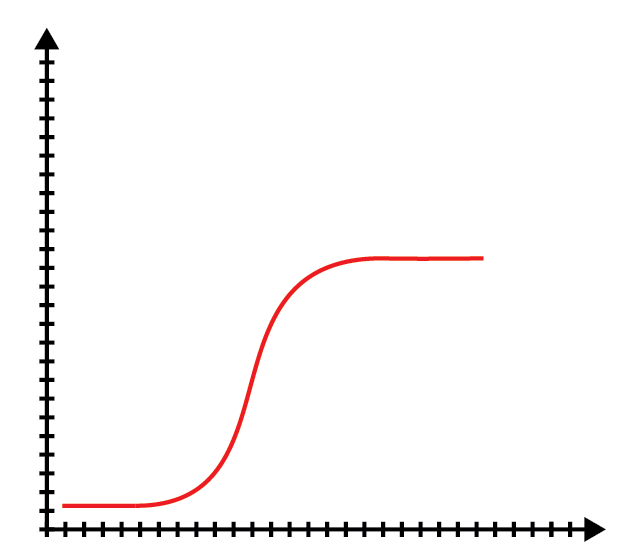
\includegraphics[width=3cm, height=3cm]{continuos_cdf}

\subsection{Binomial Distribution}
Binomial distribution expresses the discrete probability distribution of an experiment that is repeated multiple times, having only two possible outcomes: positive or negative. 
Binomial refers to the distribution having only two possible outcomes, positive or negative. 

Binomial distribution is expressed as $B(n,p)$, with n being trials and p being the probability of success. 

$ \displaystyle f(k,n,p)=\Pr(k;n,p)=\Pr(X=k)={\binom {n}{k}}p^{k}(1-p)^{n-k}$

for $k = 0, 1, 2, \ldots, n$ where, as already explained:

$ \displaystyle {\binom {n}{k}}={\frac {n!}{k!(n-k)!}}$

Binomial distribution should respect the following criteria:
\begin{itemize}
    \item Outcome is binomial (positive or negative, 1 or 0, + or - etc.).
    \item Each event is independent.
    \item The number of trials n is fixed.
    \item Success \textbackslash failure rate p is constant.
\end{itemize}

\paragraph{Binomial Distribution Overview}\mbox{} \\

\begin{itemize}
    \item Notation: $B(n,p)$
    \item Parameters: 
        \begin{itemize}
            \item $ \displaystyle n\in \{0,1,2,\ldots \} $ – number of trials 
            \item $ \displaystyle p\in [0,1] $ – success probability for each trial
            \item $ {\displaystyle q=1-p} $
        \end{itemize}
    \item Support: $ \displaystyle k\in \{0,1,\ldots ,n\}$ – number of successes 
    \item PMF: $ \displaystyle {\binom {n}{k}}p^{k}q^{n-k} $
    \item CDF: $ \displaystyle I_{q}(n-k,1+k) $ (the regularized incomplete beta function)
    \item Mean: $np$
    \item Median: $\lfloor np \rfloor$  or $\lceil np \rceil $
    \item Mode: $\lfloor (n+1)p \rfloor$  or $\lceil (n+1)p \rceil-1 $
    \item Variance: $npq$ 
\end{itemize}

\textbf{Example of a binomial distribution:} \\

According to a report, 80\% of prospects at company $\alpha$ will result in a signed contract. Each prospect is independent of each other.
It's asked to calculate the probability to close a deal from a round of 3 prospects they are working on.

Hence:
\begin{itemize}
    \item $n$ = Number of trials = 3
    \item Number of outcomes = binary positive \textbackslash negative (contract or no contract).
    \item $p$ = Probability of success = 0.8
    \item Trials are independent = yes.
    \item $k$ = Target result = 1 contract closed = 1
\end{itemize}

$ \displaystyle {\binom {n}{k}} = {\binom {3}{1}} = \frac{3!}{1!(3 - 1)!} = 3$

and then $B = 3 * (0.8^1)(1 - 0.8)^(3-1)$ = 0.096

Calculating then the values for each value of $k \in n$, hence $P\binom {n}{k}$ = P(3,0), P(3,1), P(3,2), P(3,3) we should be able to plot a chart of the distribution.


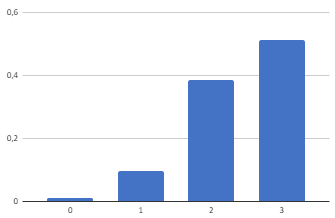
\includegraphics[width=3cm, height=3cm]{excel_chart_1}

\subsection{Bernoulli Distribution}
The Bernoulli distribution is the discrete probability distribution of a random variable which takes the value 1 with probability $p$ and the value 0 with probability $q = 1 - p$. 
Less formally, it can be thought of as a model for the set of possible outcomes of any single experiment that asks a yes-no (boolean) question. 
Such questions lead to outcomes that are boolean-valued: a single bit whose value is success, yes, true, 1 with probability $p$ and failure, no, false, 0 with probability $q = 1 - p$. 

Bernoulli distribution can be see as a specific case of binomial distribution, where:
\begin{itemize}
    \item Binomial distribution: n trials
    \item Bernoulli distribution: one trial.
\end{itemize}

It can be used to represent a (possibly biased) coin toss where 1 and 0 would represent "heads" and "tails", respectively, and $p$ would be the probability of the coin landing on heads (or vice versa where 1 would represent tails and $p$ would be the probability of tails). In particular, unfair coins would have $p \neq  1/2 $

\paragraph{Bernouilli Distribution Overview}\mbox{} \\

\begin{itemize}
    \item Notation: $X \sim B(1,p)$
    \item Parameters: 
        \begin{itemize}
            \item $ 0 \leq p \leq 1 $
            \item $ q=1 - p $
        \end{itemize}
    \item Support: $ k\in \{0,1\} $
    \item PMF: $ \displaystyle {\begin{cases}q=1-p&{\text{if }}k=0\\p&{\text{if }}k=1\end{cases}} $
    \item CDF: $ \displaystyle {\begin{cases}0&{\text{if }}k<0\\1-p&{\text{if }}0\leq k<1\\1&{\text{if }}k\geq 1\end{cases}} $
    \item Mean: $p$
    \item Median: $ \displaystyle {\begin{cases}0&{\text{if }}p<1/2\\\left[0,1\right]&{\text{if }}p=1/2\\1&{\text{if }}p>1/2\end{cases}} $
    \item Mode: $ \displaystyle {\begin{cases}0&{\text{if }}p<1/2\\0,1&{\text{if }}p=1/2\\1&{\text{if }}p>1/2\end{cases}} $
    \item Variance: $ \displaystyle p(1-p)=pq $ 
\end{itemize}

\subsection{Poisson Distribution}
Poisson distribution is a discrete probability distribution that expresses the probability of a given number of events occurring in a fixed interval of time or space if these events occur with a known constant mean rate and independently of the time since the last event.

A discrete random variable $X$ is said to have a Poisson distribution, with parameter $\lambda > 0$, if it has a probability mass function given by:

$ \displaystyle f(k;\lambda )=\Pr(X{=}k)={\frac {\lambda ^{k}e^{-\lambda }}{k!}} $

where:
\begin{itemize}
    \item k is the number of occurrences ($…k=0,1,2,\ldots) $.
    \item e is Euler's number ($ e=2.71828\ldots$)
    \item ! is the factorial function.
\end{itemize}

Poisson distribution should respect the following criteria:
\begin{itemize}
    \item The mean number of events occurring within a given interval of time or space lambda ($\lambda$) is known and assumed to be constant.
    \item Occurrences occur in an interval and are discrete and countable.
    \item Events occur independently one to another.
    \item The average rate at which events occur is independent of any occurrences (assumed to be constant).
    \item Two events cannot occur exactly at the same instant. At each atomic interval, either or one event occurs or no event occurs (it means that intervals are not overlapping).
    \item Probability is proportional to interval size. 
\end{itemize}

Some examples of Poisson distribution are:
\begin{itemize}
    \item The number of chewing gum on a single tile over a sidewalk. 
    \item The number of planes that fly over a specific house in an hour.
\end{itemize}

One of the first applications of Poisson distribution was the investigation of deaths by horse kick in soldiers in 1800. Researchers were interested in inferring the deaths by horse kick in a year.
\begin{itemize}
    \item Event = death by kick
    \item Time interval = 1 year
    \item $\lambda$ = 0.61
\end{itemize}

The number of times an event is investigated is $k$ and is assumed to be $k = 2$ (we want to calculate the probability that in a year 2 soldiers will die from a horse kick).

Hence: 

P($X = k$ where $k = 2$) = $ \displaystyle \frac {0.61^{2}e^{-0.61 }}{2!} $ = 0.101 

\paragraph{Poisson Distribution Overview}\mbox{} \\

\begin{itemize}
    \item Notation: $Pois(\lambda)$
    \item Parameters: $ \displaystyle \lambda \in (0,\infty)$ (rate)
    \item Support: $ \displaystyle k\in \mathbb {N} _{0}$ (Natural numbers starting from 0) 
    \item PMF: $ \displaystyle {\frac {\lambda ^{k}e^{-\lambda }}{k!}} $
    \item CDF: $ \displaystyle {\frac {\Gamma (\lfloor k+1\rfloor ,\lambda )}{\lfloor k\rfloor !}}$, or $\displaystyle e^{-\lambda }\sum _{j=0}^{\lfloor k\rfloor }{\frac {\lambda ^{j}}{j!}}$, \\ or $\displaystyle Q(\lfloor k+1\rfloor ,\lambda )$ \\ (for $\displaystyle k\geq 0$, where $\Gamma (x,y)$ is the upper incomplete gamma function, $ \displaystyle \lfloor k\rfloor $ is the floor function, and $Q$ is the regularized gamma function).
    \item Mean: $\lambda$
    \item Median: $ \displaystyle \approx \left\lfloor \lambda +{\frac {1}{3}}-{\frac {1}{50\lambda }}\right\rfloor $
    \item Mode: $ \displaystyle \left\lceil \lambda \right\rceil -1,\left\lfloor \lambda \right\rfloor $
    \item Variance: $ \lambda $ 
\end{itemize}

\clearpage

\section{Normal Distribution}
In statistics, a normal distribution or Gaussian distribution is a type of continuous probability distribution for a real-valued random variable. 

The general form of its probability density function is:

$\displaystyle f(x)={\frac {1}{\sigma {\sqrt {2\pi }}}}e^{-{\frac {1}{2}}\left({\frac {x-\mu }{\sigma }}\right)^{2}}$

A random variable with a Gaussian distribution is said to be normally distributed and is called a normal deviate

Normal distribution is one of the most common distribution used in business, statistics, biology, etc., since so many real-life datasets end up resembling a normal distribution (see also: Central Limit Theorem).

Normal distributions are referred to with capital letter $N$, such as $N(5,9)$ means a normal distribution with mean 5 and variance 9.

Normal distributions have unique properties of mean and standard deviation.

\paragraph{The Empirical Rule}\mbox{} \\
\mbox{} \\

The below chart helps understanding the empirical rule.

The empirical rule (also known as three-sigma rule or 68-95-99.7 rule) states that for a normal distribution, almost all observed data will fall within the range of $3 \sigma $ from the mean $ \mu $. 

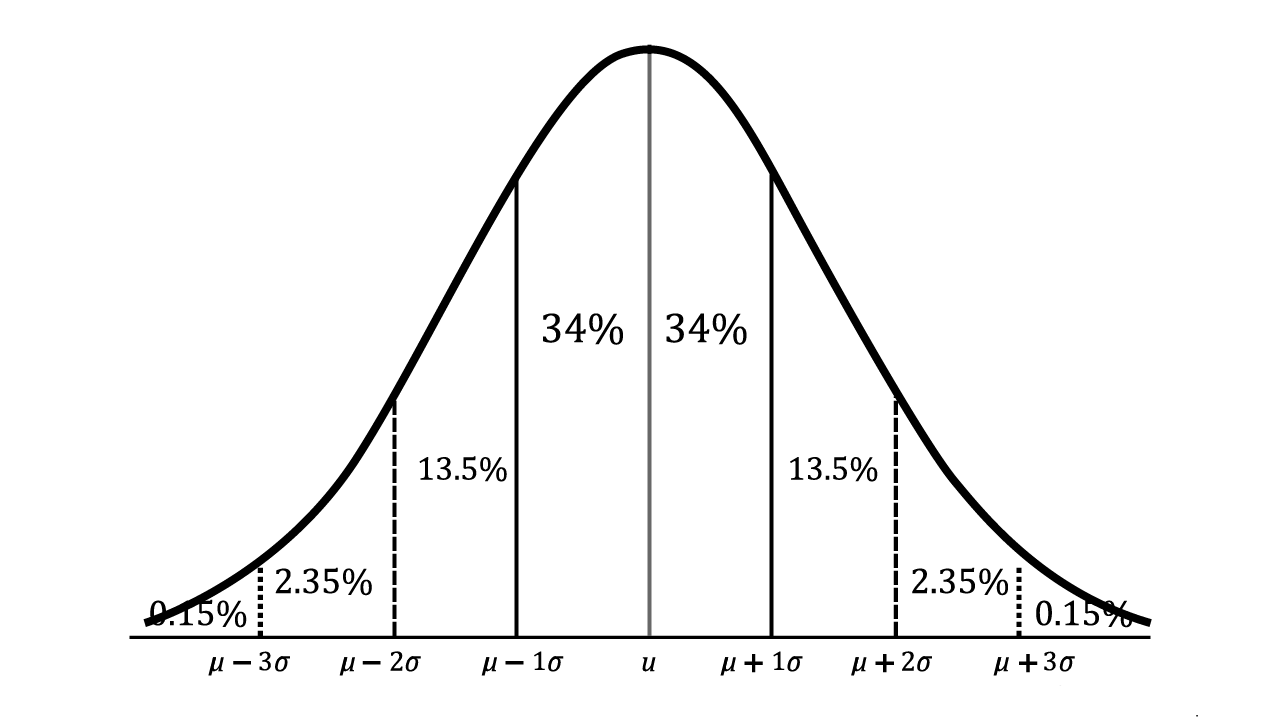
\includegraphics[width=5cm, height=3cm]{empirical}

In particular, it can be stated that:
\begin{itemize}
    \item 68\% of observations will fall within the first standard deviations ($\mu \pm \sigma $).
    \item 95\% of observations will fall within the first two standard deviations ($\mu \pm 2\sigma $).
    \item 99.7\% of observations will fall within the first three standard deviations ($\mu \pm 3\sigma $)
\end{itemize}

\subsection{Z-Score}
Z-score (even called standard score) is the number of standard deviations by which the value of an observed value or data point is above or below the mean of the distribution. Less technically, z-scores represents how a given data point is far from the mean.

Negative z-scores fall on the left of the distribution (-4 being the further) while positive z-scores fall on the right of the distribution (+4 being the further).

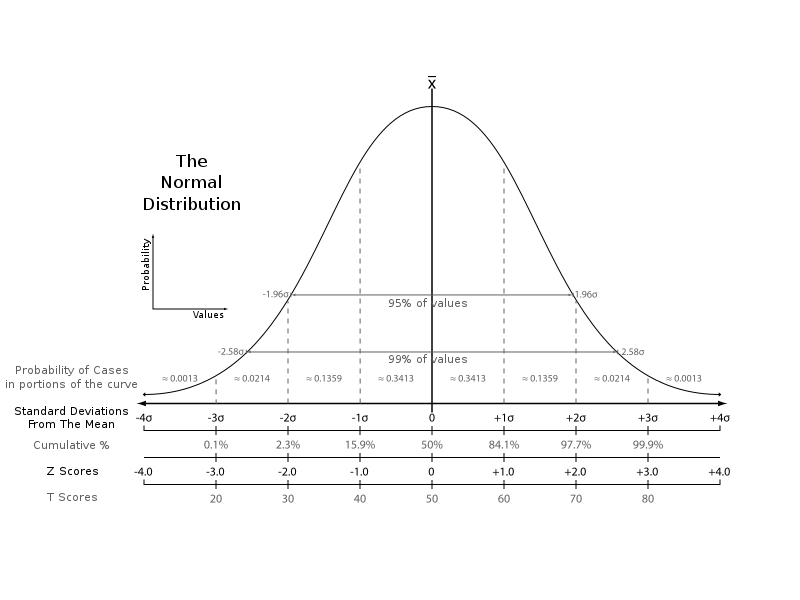
\includegraphics[width=8cm, height=6cm]{normal_distribution}

Z-score standardization formula is:

$\displaystyle Z={\frac {X-\mu }{\sigma }}$

\subsubsection{Z-Tables}
A z-table, or standard normal table, reveals what percentage of values fall below a certain z-score in a normal distribution. It allows to translate specifics z-scores to their statistic relevance in a normal distribution.

The table has z decimal values on the row header, and hundredth values on the table header. First turn your data into a normal distribution. Then find the matching z-score to the left of the table and align it with the z-score at the top of the table. The result gives you the probability. 

The image below shows the probability for a z-score of 1.2 + 0.5 = 1.25, that is 0.89435.

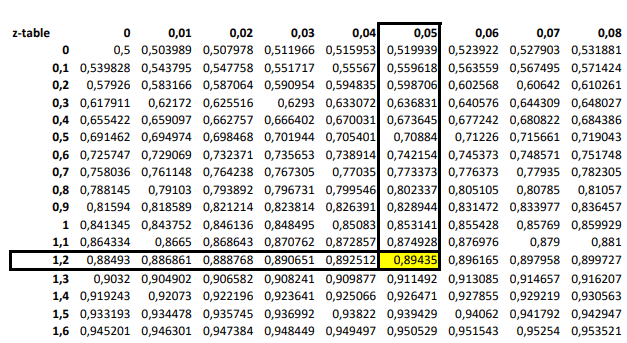
\includegraphics{z-table}

A z-table can also be created from the ground-up, in example: 
\begin{enumerate}
    \item with Excel using the formula:
    \begin{enumerate}
        \item =+NORM.S.DIST($A2+B$1;TRUE), having "A" column = [0, 0.1, 0.2, …, 3.4] and row 1 = [0, 0.01, 0.02, …, 0.09]
    \end{enumerate}
    \item with a programming language, such as R or Python (here is script for generating a z-table in Python: \href{https://gist.github.com/carloocchiena/f65e1381a30004352561a606ee0ba51a}{gist.github.com/carloocchiena/})
\end{enumerate}

\subsection{Normality Test}
In theory, a normal distribution follows precisely a Gaussian curve. But real world data is rarely so precise and could be the case we may be willing to test if the distribution we are working with is effectively normal.

Normality tests are used to determine if a data set is well-modeled by a normal distribution and to compute how likely it is for a random variable underlying the data set to be normally distributed. 

Normality tests return a probability of normality. More specifically, these tests operate using a hypothesis paradigm, where you posit an hypothesis that your particular data sample is normally distributed. 

Normality tests are such as:
\begin{itemize}
    \item D'Agostino's K-squared test.
    \item Jarque–Bera test.
    \item Anderson–Darling test.
    \item Kolmogorov–Smirnov test.
    \item Shapiro–Wilk test.
\end{itemize}

\subsection{Skewed Distribution (Skewness)}
Skewness is a measure of the asymmetry of the probability distribution of a random variable in respect to the mean of the distribution. 

Would be useful to remember that for a symmetric distribution, and, specifically, for a normal distribution, median = mean = mode.

\textbf{Negative Skew} \\
The left tail is longer; the mass of the distribution is concentrated on the right of the figure. The distribution is said to be left-skewed, left-tailed, or skewed to the left, despite the fact that the curve itself appears to be skewed or leaning to the right; left instead refers to the left tail being drawn out and, often, the mean being skewed to the left of a typical center of the data. A left-skewed distribution usually appears as a right-leaning curve.

\textbf{Positive Skew} \\
The right tail is longer; the mass of the distribution is concentrated on the left of the figure. The distribution is said to be right-skewed, right-tailed, or skewed to the right, despite the fact that the curve itself appears to be skewed or leaning to the left; right instead refers to the right tail being drawn out and, often, the mean being skewed to the right of a typical center of the data. A right-skewed distribution usually appears as a left-leaning curve

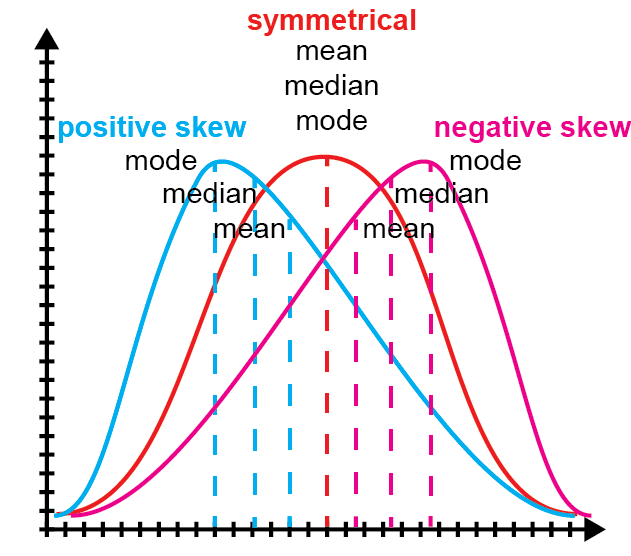
\includegraphics[width=5cm, height=5cm]{skew}

\subsection{Kurtosis}
While skewness refers to the tendency of a distribution to propagate in respect to its mean, \textbf{kurtosis} measures the sharpness of the curve in respect of its distribution. 

It can also be stated more simply that skewness represents the vertical distance of the curve from a normal distribution, while kurtosis represents the horizontal distance of the curve from a normal distribution.    

\begin{itemize}
    \item \textbf{Skewness}: lack of symmetry in the distribution.
    \item \textbf{Kurtosis}: height and sharpness of the central peak.
\end{itemize}

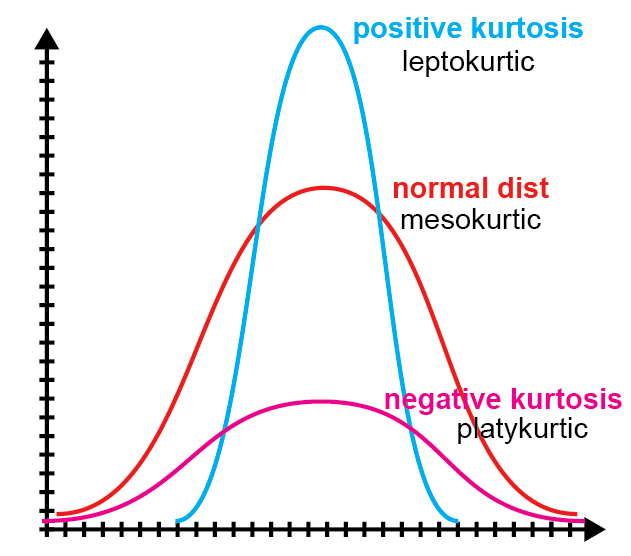
\includegraphics[width=5cm, height=5cm]{kurtosis}

\subsection{Standard Normal Distribution}
The standard normal distribution, also known as the z-distribution (Z), is a particular case of normal distribution. Standard Normal Distribution has a mean = 0 and the standard deviation = 1.

$Z = N(0,1)$

Any normal distribution can be standardized by converting its values into z scores. Z scores tell you how many standard deviations from the mean each value lies.

\clearpage

\section{Sampling}
Sampling is the selection of a subset (a \textbf{sample}) of individuals from within a statistical \textbf{population} to estimate characteristics of the whole population. Statisticians attempt to collect samples that are representative of the population in question. Sampling has lower costs and faster data collection than measuring the entire population and can provide insights in cases where it is infeasible to measure an entire population.

Sampling allows to test a hypothesis about general characteristics of a population.
Samples are used to make inferences about a population. 

One can think of sampling as grabbing data instances from a larger data distribution. 

\subsection{Sampling Methodologies}
The representativeness of the selected sample is a crucial element in creating a good sampling. Therefore, there are different types of sampling that can be chosen appropriately according to the characteristics of the population.

Some of the discriminating criteria in choosing a sampling method may be:
\begin{itemize}
    \item Nature and quality of the frame.
    \item Availability of auxiliary information about units on the frame.
    \item Accuracy requirements, and the need to measure accuracy.
    \item Whether detailed analysis of the sample is expected.
    \item Cost/operational concerns.
\end{itemize}

In general terms, it can be stated that a good sampling is:
\begin{itemize}
    \item Representative of the population.
    \item Unbiased. 
\end{itemize}
 
\subsubsection{Simple Random Sample (SRS)}
A simple random sample (or SRS) is a subset of individuals (a sample) chosen from a larger set (a population) in which a subset of individuals are chosen randomly, all with the same probability. It is a process of selecting a sample in a random way.

\subsubsection{Systematic Random Sample}
Systematic random sample is a subclass of SRS. Every member of the population is labeled with a number, and the sample is picked using a fixed interval (i.e. one out of every 10 members).

\subsubsection{Stratified Random Sample}
Stratified random sample is a subclass of SRS, where the population can be further classified into subpopulations. Subpopulations can’t overlap and they should be proportional in order for the sample to be relevant. 

\subsubsection{Clustered Random Sample}
Clustered random sample is a sampling methodology that can be used whenever the population can be aggregated into mutually homogeneous yet internally heterogeneous groupings. 
After the population is divided into clusters, then a SRS is performed on each cluster.
It’s a sampling method often used in marketing research.

\subsection{Central Limit Theorem}
In probability theory, the central limit theorem (CLT) establishes that, in many situations, when independent random variables are summed up, their properly normalized sum tends toward a normal distribution around the mean of the original dataset even if the original variables themselves are not normally distributed.

It implies that probabilistic and statistical methods that work for normal distributions can be applicable to many problems involving other types of distributions.

The CLT establishes a relationship between the data from the whole population (parameters) and the data from the sample (statistics). 

\begin{itemize}
    \item The mean of the distribution of sample means is the \textbf{expected value of $M$} and is always equal to the population mean $\mu$.
    \item The standard deviation of the distribution of sample means is \textbf{the standard error of $M$} (SE) and is computed by: $\sigma{M} = \frac{\sigma}{\sqrt{n}}$. As the sample size increases, the error decreases.  As the sample size decreases, the error increases.  At the extreme, when n = 1, the error is equal to the standard deviation.
    \item The shape of the distribution of sample means tends to be normal. It is guaranteed to be normal if either: 
    \begin{itemize}
        \item The population from which the samples are obtained is normal.
        \item The sample size is n = 30 or more.
    \end{itemize}  
\end{itemize}

\subsubsection{Sampling Distribution of the Sample Mean}
The distribution of sample means is defined as the set of means from all the possible random samples of a specific size (n) selected from a specific population. 

If repeated random samples of a given size n are taken from a population of values for a quantitative variable, the mean of all sample means is population mean.

$\bar{x} = \mu $

\paragraph{More on mean of the sampling being equal to the mean of the population}\mbox{} \\
\mbox{} \\
This statement can leads to wrong assumptions - since the mean of the sample typically is not equal to the mean of the population \textbf{unless samples are taken listing all the possible samples over the population (combinations)}.

The idea is that when we think of taking a sample, there are a large number of possible samples, from which we will choose just one. However, we need to imagine having all the samples available, and knowing the mean of each one. This list of all the possible sample means makes up the distribution of the sampling means (“the sampling distribution of the means”). Now, this distribution itself has a mean, which is how we get the somewhat confusing phrase “mean of means.”

So, while the mean of one sample is an estimate of the population mean and rarely equal to it, the mean of (all the means of all the possible samples), is exactly equal to the population mean. This is the basis of an important result in statistical theory, that the sample mean is an unbiased estimator of the population mean. There are other candidates for an estimator of the population mean, such as the median, the mode, or the geometric average. While they might be unbiased in certain situations, none of them are “in general” an unbiased estimator of the mean, like the sample mean is.\footnote{This explanation has been provided in an online debate from Dwight Galster, Statistics PhD from NDSU.}

\paragraph{Finite Population Correction Factor (FPC)}\mbox{} \\
\mbox{} \\
Finite Population Correction Factor (FPC) is used to adjust sampling bias whenever sampling is done without replacement and over more than the 5\% of a finite population (both frequent real case scenarios).

\textbf{Example}: you have to apply FPC if picking 600 people (>5\%) from a city telephone address book of 10’000 members (population is finite and whenever a person is picked from the list, can’t be picked again).

$FPC = \sqrt{\frac{N -n}{N - 1}}$

To apply a finite population correction, multiply it by the standard error that you would have originally used.

For example, the standard error of a mean is calculated as:

$\sigma{M} = \frac{\sigma}{\sqrt{n}}$

By applying the finite population correction, the formula becomes:

$\sigma{M} = \frac{\sigma}{\sqrt{n}}\sqrt{\frac{N -n}{N - 1}}$

\subsection{The Student's T-Distribution}
Student's t-distribution a family of continuous probability distributions that arise when estimating the mean of a normally distributed population in situations where the sample size is small and the population's standard deviation is unknown.

The t-distribution was developed by English statistician William Sealy Gosset. 
At the time (1912) he published more than 20 academic papers, mostly using the pseudonym “Student”.
The t-distribution was originally called “Test of statistical significance” or “Student’s z” (for its similarity to Z distribution).
In the end he could have called it “Gosset distribution”, but he passed to history as “Student”. 

The formula to calculate the T-distribution is:

$t= \frac{(\bar{x} - \mu)}{s/\sqrt{n}}$

where:
\begin{itemize}
    \item $\bar{x}$ is the sample mean.
    \item $\mu$ is the population mean.
    \item $s$ is the standard deviation.
    \item $n$ is the size of the given sample.
\end{itemize}

\subsubsection{Degrees of freedom (DF)}
The number of degrees of freedom is the number of values in the final calculation of a statistic that are free to vary (independent, known, available data).

Degrees of freedom (DF) is equal to the size of the sample n minus 1.

$DF = n - 1$

The explanation for this lies in the fact that the punctual features of a dataset can be computed backward knowing the global features of the dataset.
For example, having a dataset of 15 elements, and knowing the mean, we are free to delete one of these values, since knowing the mean we are able to calculate it backwards.
But what happens if, for example, we delete two values? We are able to trace the global value of the two variables but not to assign their value in a timely and independent way.
That is why DF is calculated as $n - 1$.

\subsubsection{T-Score}
The T-distribution (and those associated T-score values) is used in hypothesis testing
 when determining if one should reject or accept the null hypothesis.

Values of T-score have to be compared on a T-table\footnote{https://www.sjsu.edu/faculty/gerstman/StatPrimer/t-table.pdf} with a process similar to the Z-scores.

\paragraph{When to use Z-distribution and when T-distribution?}\mbox{} \\
\mbox{} \\
\begin{itemize}
    \item If sample < 30, t-distribution will provide a more accurate value.
    \item If sample > 30, z-distribution will provide a more accurate one.
\end{itemize}

\subsection{Confidence interval for the mean}




\end{document}




